\documentclass[a4paper]{article}

\usepackage[english]{babel}
\usepackage[utf8]{inputenc}
\usepackage{hyperref}
\usepackage{amsmath}
\usepackage{float}
\usepackage[margin=0.5in]{geometry}
\usepackage{graphicx}
\usepackage[colorinlistoftodos]{todonotes}
\usepackage{subfig}
\usepackage{booktabs}
\usepackage{epstopdf}


\title{10701 Project Final Report \\
\Large{American Epilepsy Society Seizure Prediction Challenge}}

\author{Revanth Bhattaram (rbhattar) \\ 
Archit Karandikar (akarandi) \\ 
Vipul Singh (vipuls)}

\date{\today}

\begin{document}
\maketitle

\section{Introduction}

\subsection{Background and Motivation}
Epilepsy afflicts nearly 1\% of the world's population, and is characterized by the occurrence of spontaneous seizures. For many patients, anticonvulsant medications can be given at sufficiently high doses to prevent seizures, but patients frequently suffer side effects. For 20-40\% of patients with epilepsy, medications are not effective; and even after surgical removal of epilepsy-causing brain tissue, many patients continue to experience spontaneous seizures. Despite the fact that seizures occur infrequently, patients with epilepsy experience persistent anxiety due to the possibility of a seizure occurring.

Seizure forecasting systems thus have the potential to help patients with epilepsy lead more normal lives. In order for EEG-based seizure forecasting systems to work effectively, computational algorithms must reliably identify periods of increased probability of seizure occurrence. If these seizure-permissive brain states can be identified, devices designed to warn patients of impeding seizures would be possible. Patients could avoid potentially dangerous activities like driving or swimming, and medications could be administered only when needed to prevent impending seizures, reducing overall side effects.

\subsection{The Problem} 
Our project is based on a \href{https://www.kaggle.com/c/seizure-prediction}{kaggle} competition wherein the task is to distinguish between ten minute long data clips covering an hour prior to a seizure, and ten minute iEEG clips of interictal activity. The goal of the competition is to demonstrate the existence and accurate classification of the preictal brain state in dogs and humans with naturally occurring epilepsy.

\subsection{Metrics} 
Being a Kaggle contest, one well-defined metric for success is the score provided by the contest platform. For each clip in the test set, we predict a real-valued probability that a given clip is preictal. The score is computed based on the area under the \href{http://en.wikipedia.org/wiki/Receiver_operating_characteristic}{ROC} curve (AUC). \\

We have also developed a K-fold cross-validation framework which helps us judge performance via F-score. We want high recall on preictal segments, so we use weighted F-score. The rationale behind this is that for our use-case, it is important for us to not have false negatives (a patient should always be made aware before a seizure).

\subsection{Goals}
The minimum goal is to achieve good recall because that would mean that we are able to predict preictal states correctly and hence enable provision of relief to epilepsy-afflicted patients. We would specifically want to beat the bonehead model. \\
From the perspective of learning, we aim to apply various learning/classification algorithms suited to our problem, and study their pros and cons, and why some of them work well and others don't, based on our understanding of the data.

\section{Dataset}
Intracranial EEG was recorded from dogs with naturally occurring epilepsy using an ambulatory monitoring system. Datasets from patients with epilepsy undergoing intracranial EEG monitoring to identify a region of brain that can be resected to prevent future seizures are also included in the contest. These are available at \url{https://www.kaggle.com/c/seizure-prediction/data}. 
\begin{itemize}
\item \textbf{Training Data Set} : This is organized into one hour sequences of ten-minute iEEG clips labeled `Preictal' for pre-seizure data segments, or `Interictal' for non-seizure data segments. The interictal activity data, in the case of canines, is recorded at least a week before and after a seizure. For human training data, the interictal training data is recorded at least 4 hours before and after a seizure. The preictal activity data is recorded one hour prior to a seizure with a 5 minute offset.
\item \textbf{Test Data Set} : For each subject (5 dogs and 2 patients), it consists of 10 minute iEEG clips which are
provided in random order. 
\end{itemize}

\subsection{Preliminary Analysis}
\label{prelim}
The first step taken was to plot the EEG sample values for the various subjects/electrodes and see if we could derive information out of them. An example of such a plot is shown in Figure~\ref{fig:eeg}.

\begin{figure}
  \centering
    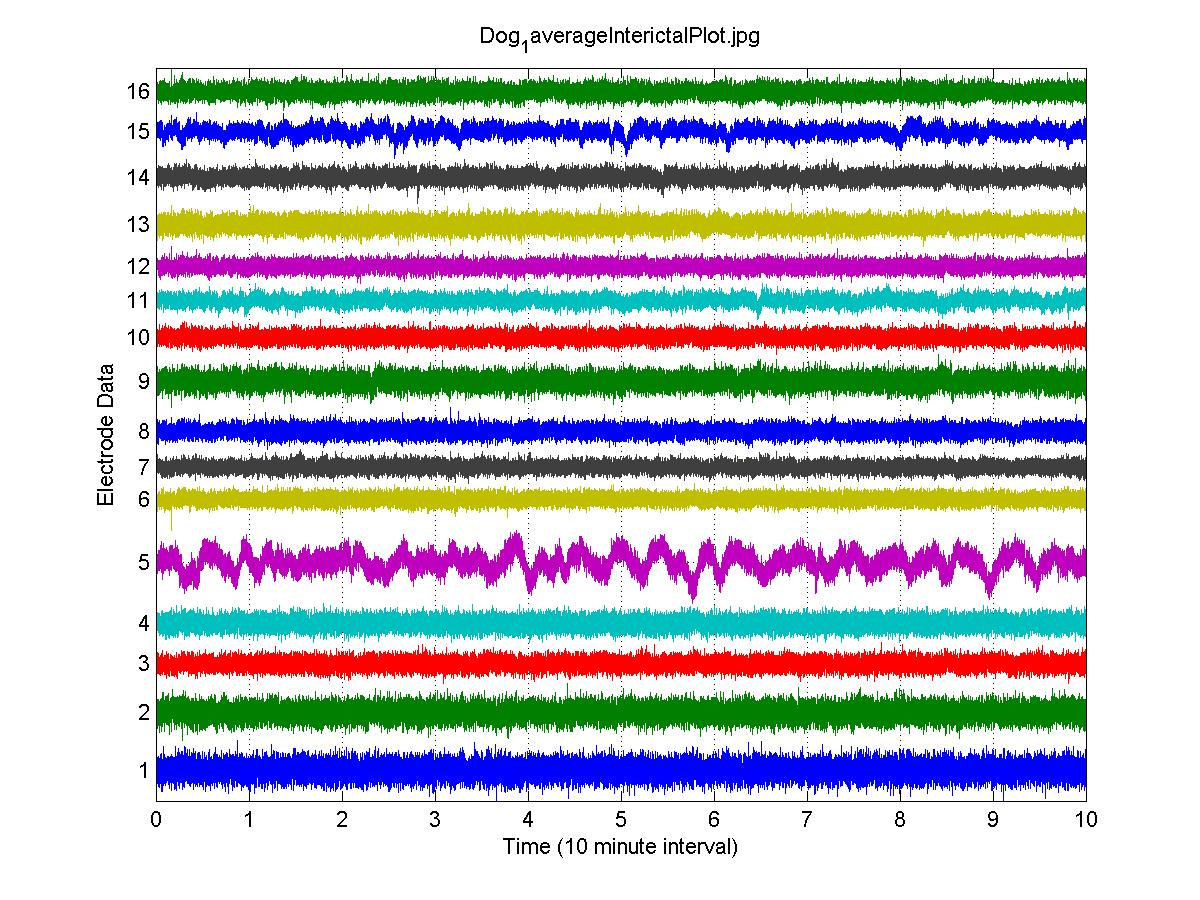
\includegraphics[width=0.8\textwidth]{EEGPlot.jpg}
  \caption{Plot of electrode-wise average EEG signal activity for a 10-minute segment. x-axis represents time in minutes}
  \label{fig:eeg}
\end{figure}

Plots for interictal and preictal data segments were made in an attempt to see if there were any major differences that we could spot. Although, we weren't able to derive too much information from these plots (other than the existence of outlier data segments), it did serve as a motivation to try Fourier methods (described later on).

\subsection{Extracting Basic Features}
We managed to calculate basic statistics like the mean/variance of each data segment over all subjects. This data is used to construct the feature vectors in our bonehead model.

The general trend that we observed was that the variance of the preictal data was lesser than that of the interictal data. This is illustrated in the following heatmap:

\begin{figure}[H]
    \centering
    \subfloat[interictal]{{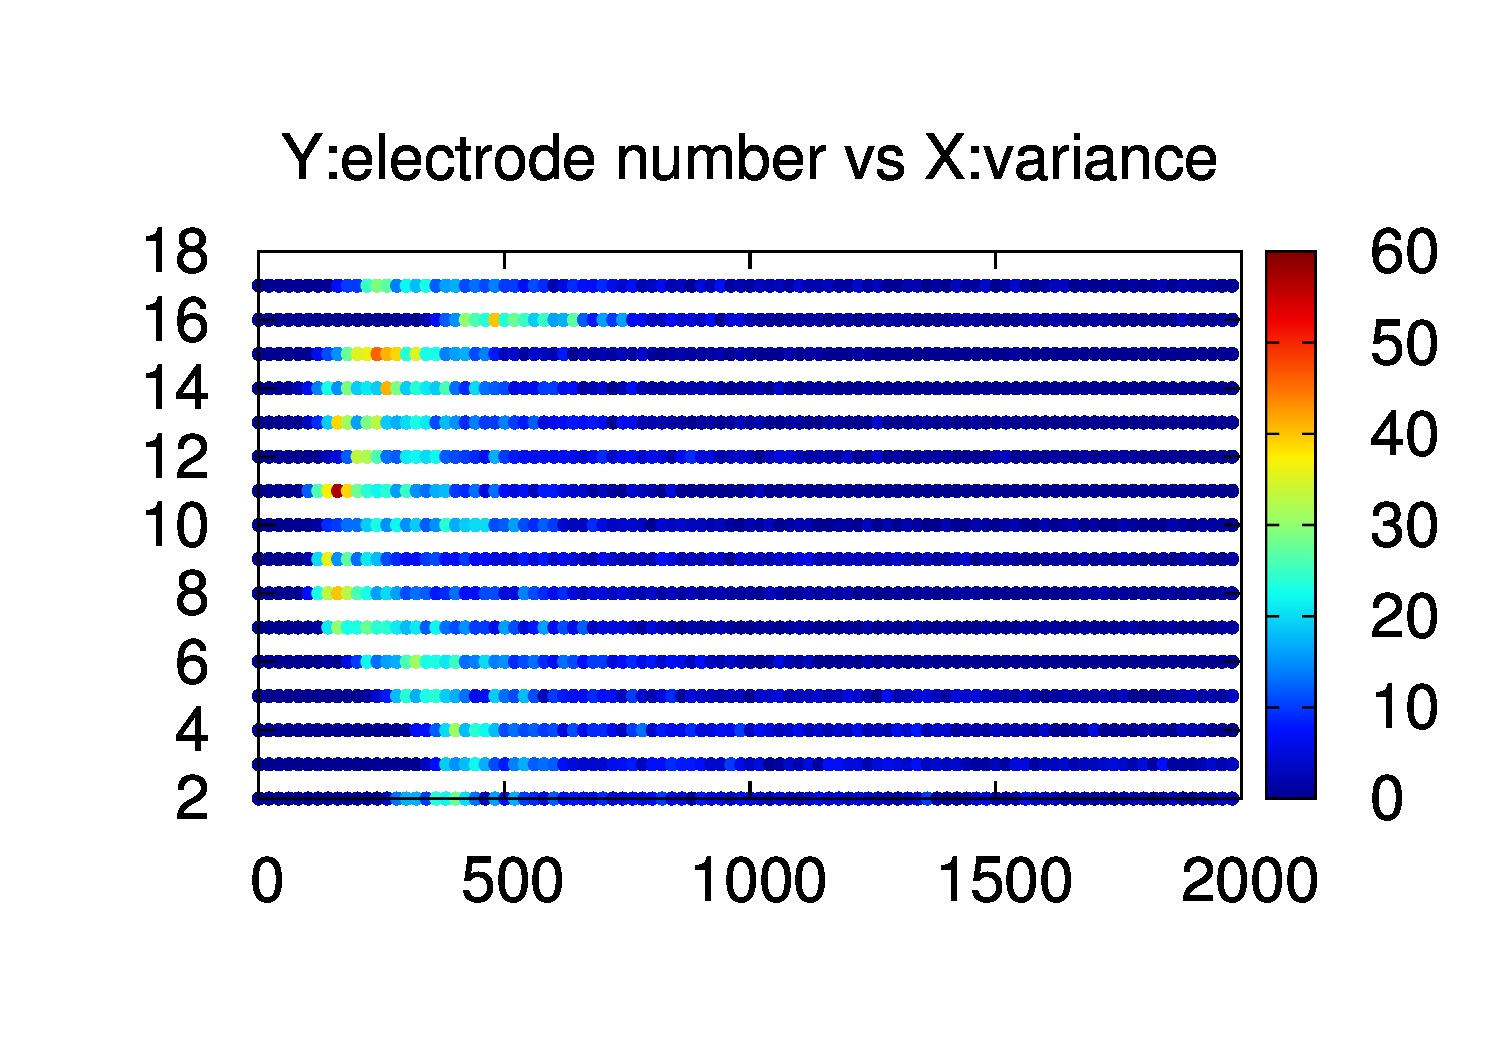
\includegraphics[width=0.4\linewidth]{Dog_2_interictal_heatmap.jpg} }}%
    \qquad
    \subfloat[prerictal]{{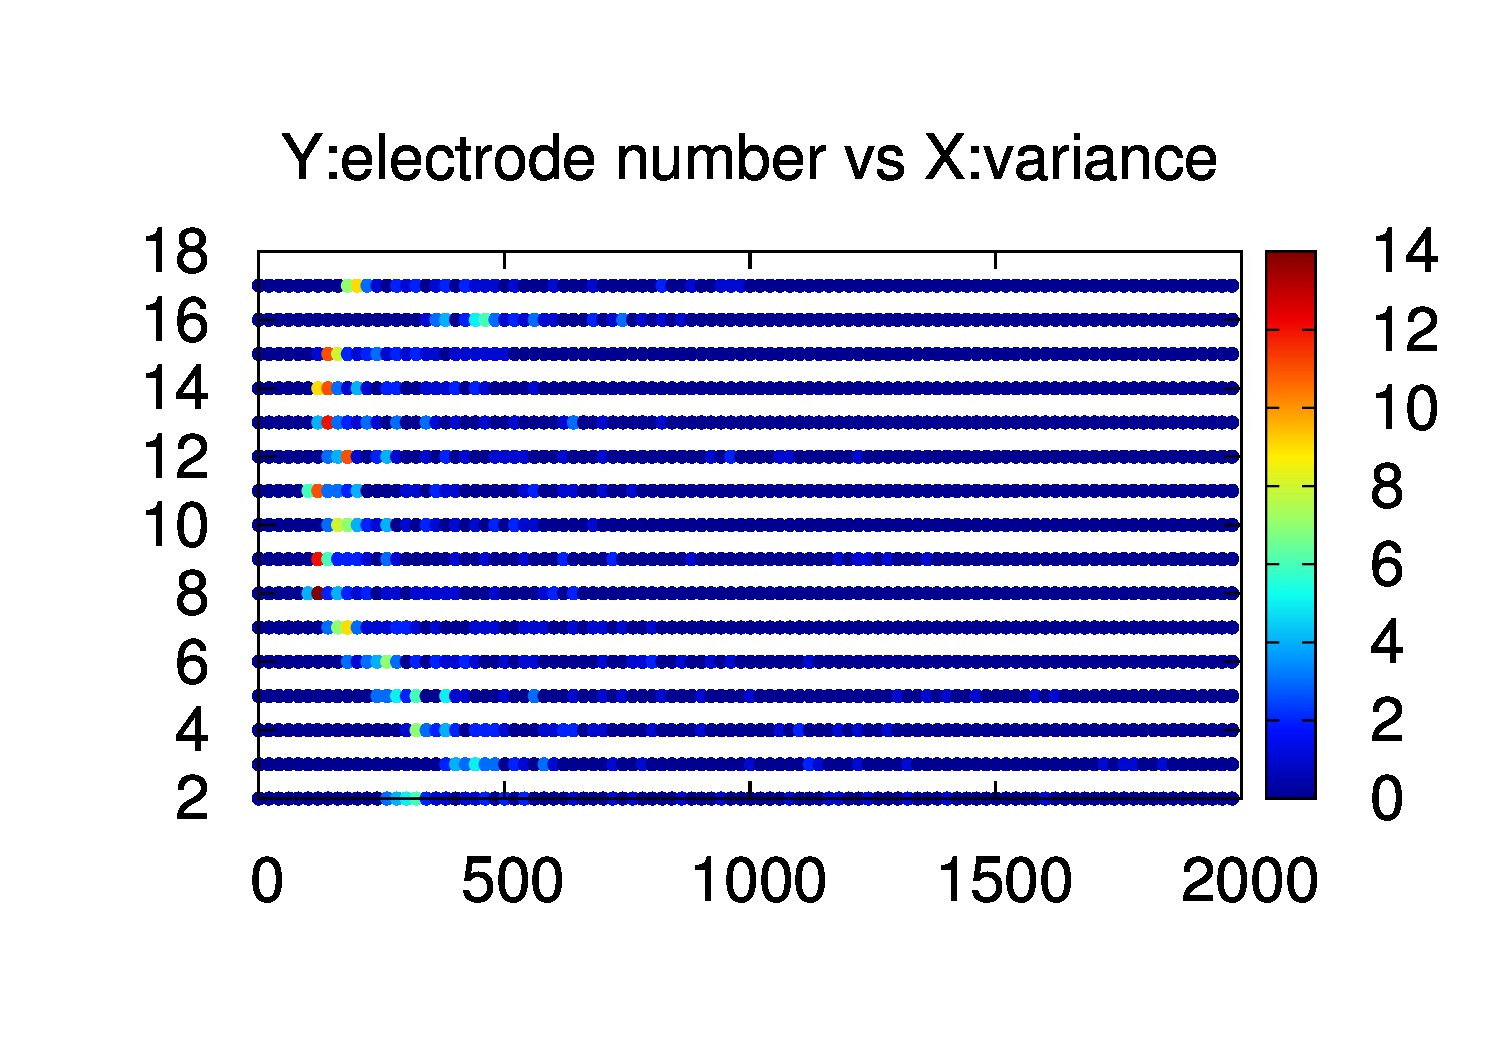
\includegraphics[width=0.4\linewidth]{Dog_2_preictal_heatmap.jpg} }}%
    \caption{Heat maps showing the distibution of variance for every electrode for Dog  2}%
    \label{fig:heatvar}%
\end{figure}

\subsubsection{Trying To Find A Correlation}

Another statistic that we managed to calculate was the covariance matrix of data segments. Following that, we calculated the correlation coefficient matrix for each data segment and tried to see if they would give us any information about correlation between electrodes. To observe this, we used heatmaps (Figure \ref{fig:corrMatrix}) for interictal data and preictal data.

\begin{figure}[H]
    \centering
    \subfloat[Interictal]{{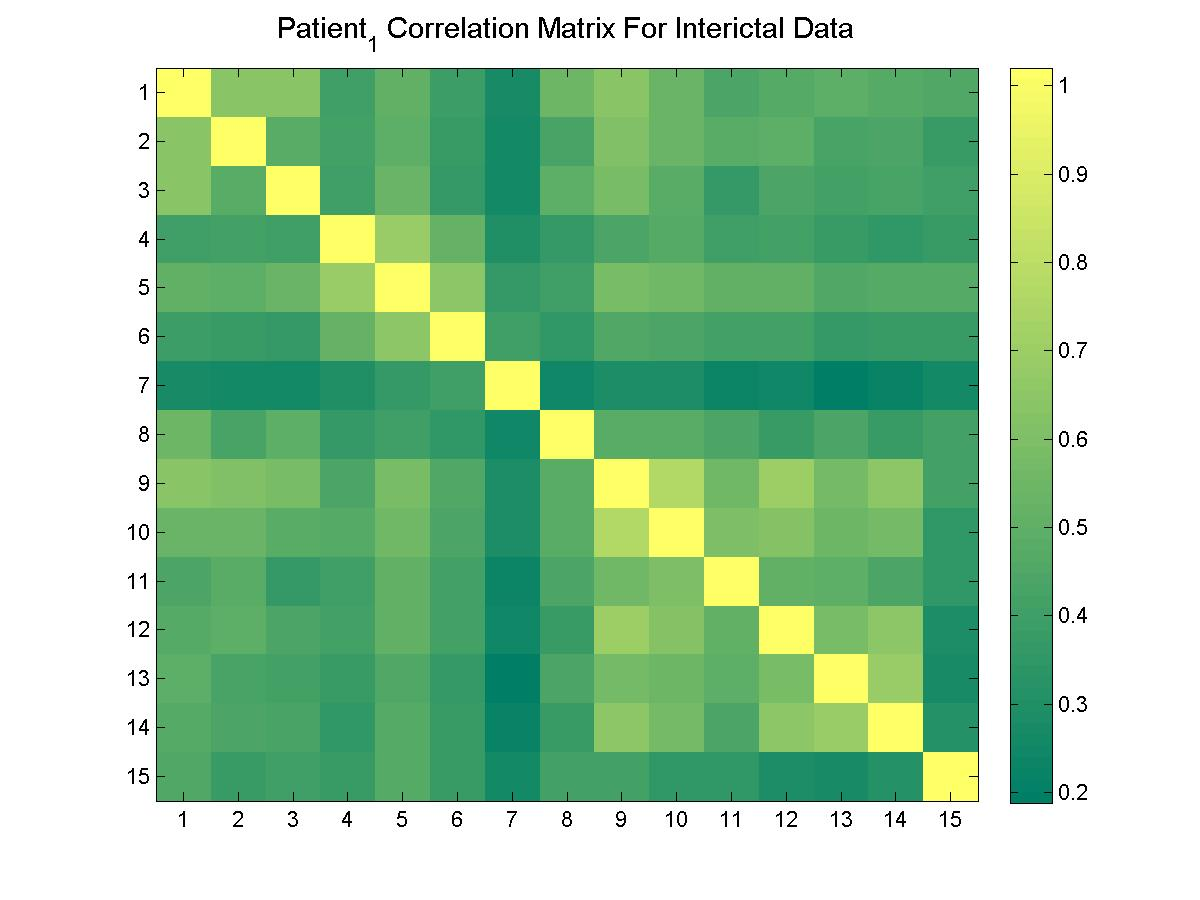
\includegraphics[width=0.4\linewidth]{InterictalCorrelation.jpg} }}%
    \qquad
    \subfloat[Preictal]{{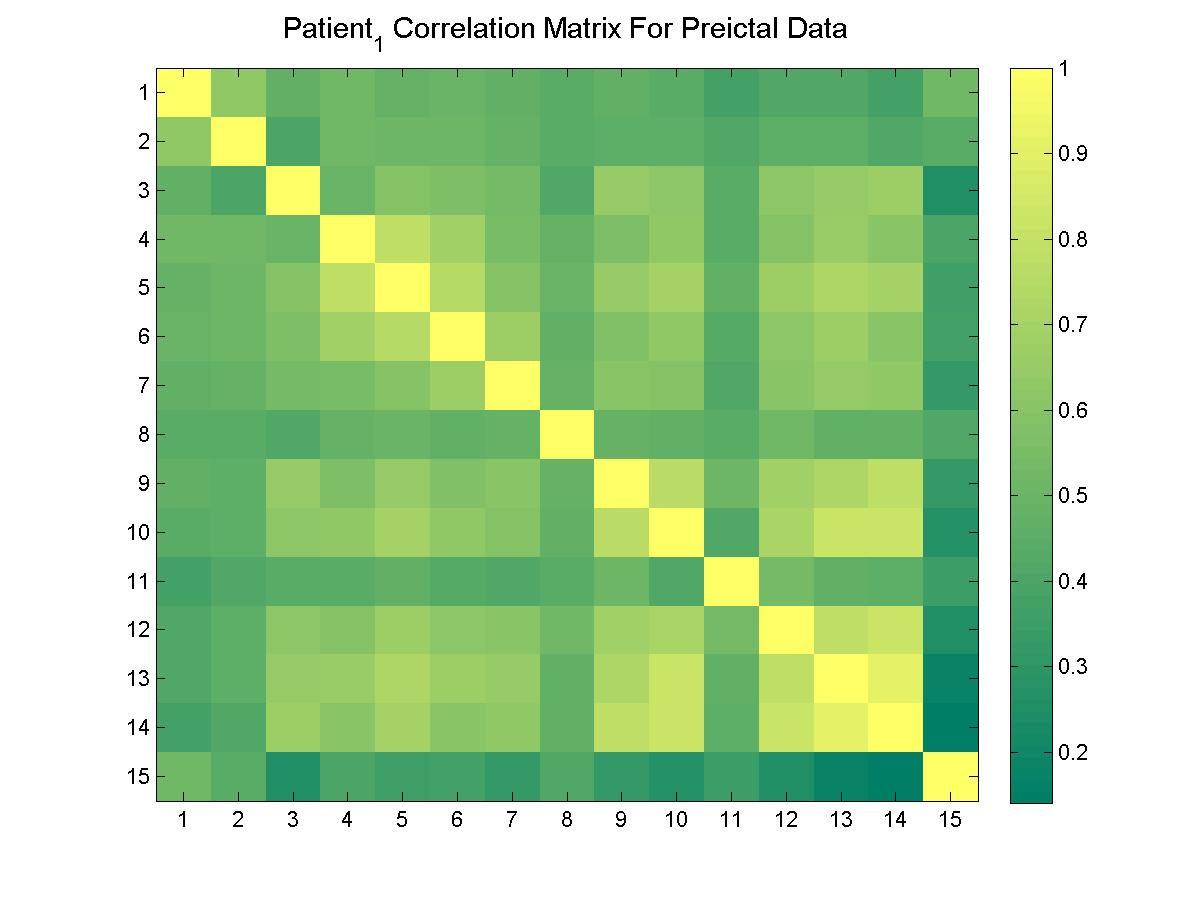
\includegraphics[width=0.4\linewidth]{PreictalCorrelation.jpg} }}%
    \caption{Correlation Coefficient Matrix for the two states}%
    \label{fig:corrMatrix}%
\end{figure}

In the heatmap plots, a box with a more intense color (according to the color scale) would correspond to a pair of electrodes that have a high correlation coefficient (which is why the boxes in the diagonal have the most intense colors). Observe how the plot changes when we move from interictal to preictal. It becomes 'brighter'.  This means that there is more correlation between pairs of electrodes in the preictal state when compared to the interictal state. This difference gives us motivation to look for bivariate features which will be able to distinguish between preictal and interictal states better than a normal univariate feature. This assumption is supported in a study that has been carried out in \cite{lecun}.

Using these simple features, we built a Naive Bayes classifier (which we call the Bonehead Model). The results are shown in Table \ref{tab:bonehead}. To improve on the results obtained, we ventured into extracting features that are more data-driven and hence can be expected to help build better classifiers. We also explored another avenue, namely treating the problem as a 7-class one instead of binary classification. These are explained in the following section.

\section{Proposed Methods and Features}

\subsection{7-Class classification}
The training data is labeled with sequence numbers which identify the 10-minute interval within an hour. One of the approaches that we tried was separating the preictal class into 6 classes corresponding to the 6 sequence types. The rationale underlying this model was that one would expect the ``preictalness" of a preictal segment to increase markedly with time in the hour before the seizure unlike the ``interictalness" of an interictal segment. We conducted several analyses of the test data in an attempt to find evidence to support this intuition. Figure \ref{fig:meanvar} demonstrates the results of two of our experiments:

\begin{figure}[H]
    \centering
    \subfloat[Mean]{{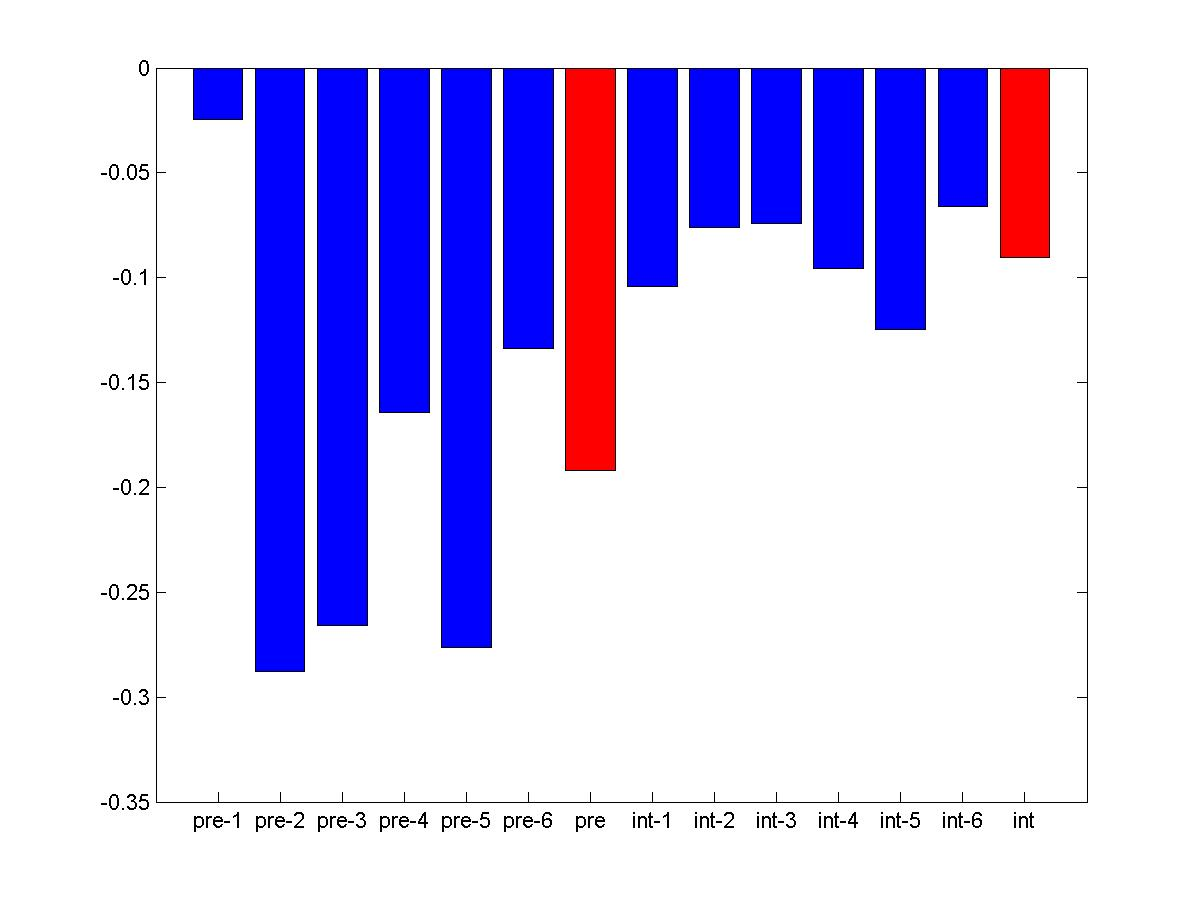
\includegraphics[width=0.4\linewidth]{Dog_2_Electrode_4_mean.jpg} }}%
    \qquad
    \subfloat[Variance]{{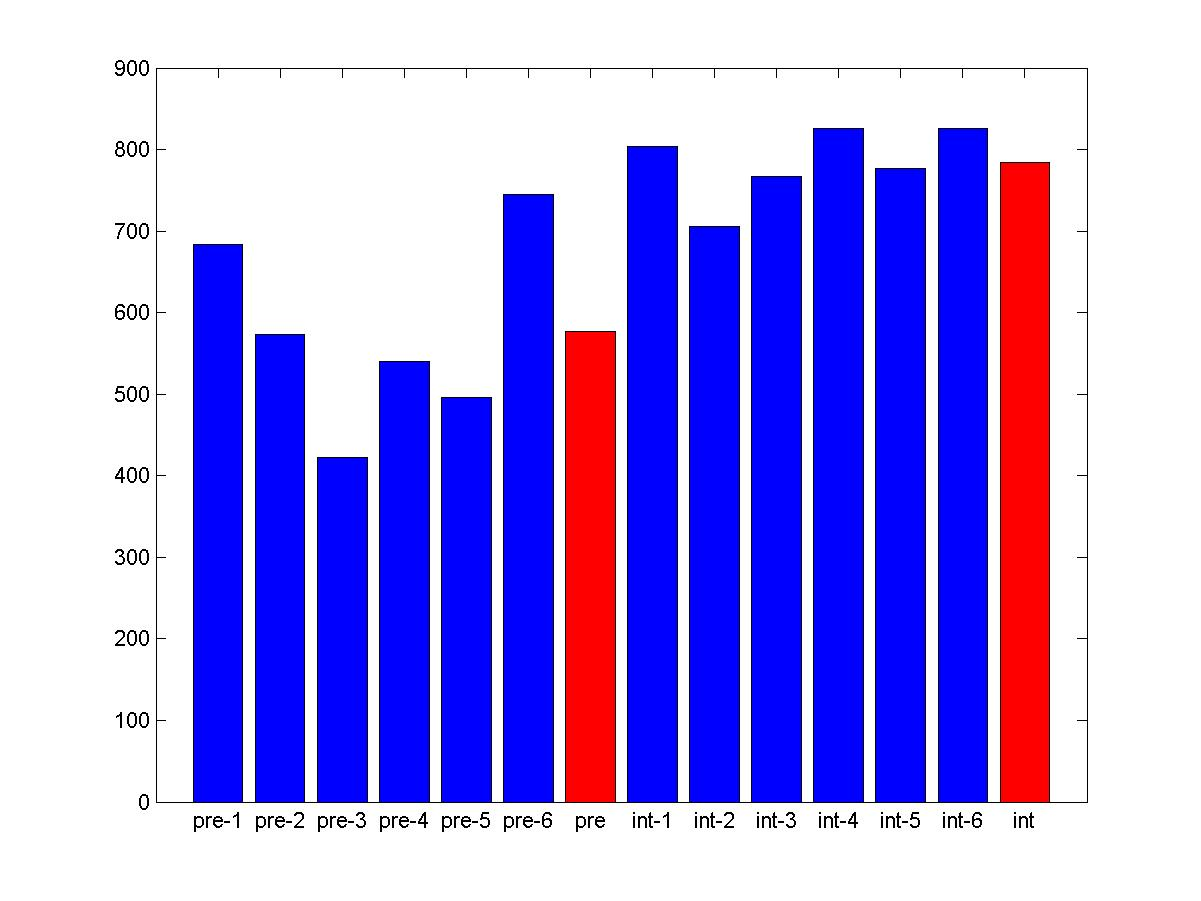
\includegraphics[width=0.4\linewidth]{Dog_2_Electrode_4_var.jpg} }}%
    \caption{Segment-specific (averaged) mean and variance for Dog 2 and Electrode 4}%
    \label{fig:meanvar}%
\end{figure}

This analysis showed us the general trend of interictal variances being higher than preictal variances. We also observed that in general, the 6 interictal means for a given subject-electrode pair were clustered together as compared to the preictal means. However we did not observe any clear trend across all subjects which could help us differentiate between the 6 preictal classes.

In contrast, the Fourier analysis presented in the following section showed clear patterns which could be used to differentiate between preictal and interictal data. Hence, we plan to focus on binary classification with Fourier Analysis in the future although we have not completely ruled out the 7-class classification model.

\subsection{Fourier Analysis}
As observed from the EEG graphs in \ref{prelim}, the signals from each electrode in a segment are quite periodic. Hence, we can apply Fourier Analysis on these signals to obtain amplitude spectrum over a range of frequencies. Below, we summarize our experiments relating to this: 

\subsubsection{Principal Frequencies}
We calculated the principal frequencies, i.e., the ones with maximum amplitude in the Fourier spectrum, for each electrode in each segment. Then, we took mean over all electrode-wise principal frequencies for a subject, and were able to get good separation between preictal and interictal segments. As an example, for Dog\_1, we obtain the mean principal frequencies for the 16 electrodes as shown in Figure  \ref{fig:d1prin}

\begin{figure}
  \centering
   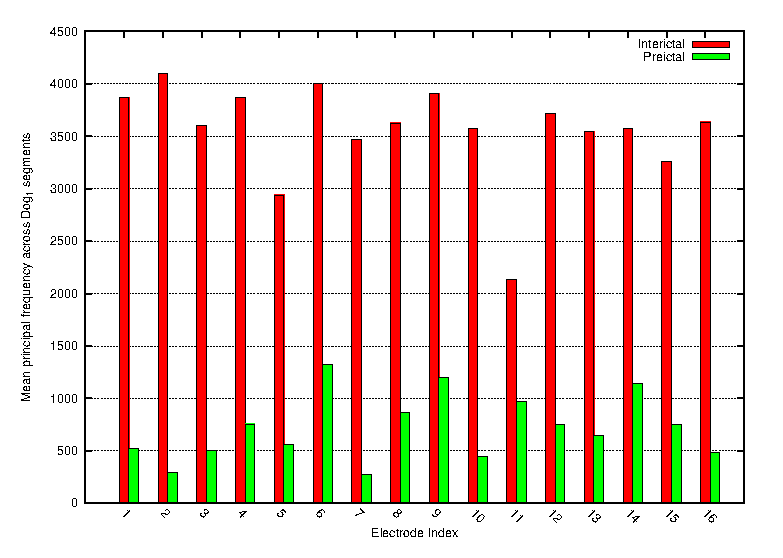
\includegraphics[width=0.8\textwidth]{dog1principalfreqs.eps}
  \caption{Electrode-wise Mean Principal Frequency for Dog1 Interictal and Preictal segments}
  \label{fig:d1prin}
\end{figure}
On taking a closer look at the individual principal frequencies, we observe that there are some huge outliers, in the range of $10^{5}$ to $10^{6}$, while the smaller values are all clustered in ranges of around 0-200 Hz, for both preictal as well as interictal segments. This is the reason why the mean principal frequencies for interictal segments reach values upto 4 kHz.

\subsubsection{Outlier Detection}
To deal with the above-mentioned issue of outliers, we filtered the electrode-wise principal frequencies and retained only those segments where the frequencies were less than 10 times the average values for their respective electrodes. On doing so, we observed that the principal frequencies for both interictal as well as preictal data had clustered in the range 0-100 Hz. This is depicted via the sample heatmaps in figure \ref{d1freq}. Hence, just the set of principal frequencies doesn't seem to be a good distinguishing feature. We have, in a way, aggregated a 10-minute signal into one value, which leads to loss of information.

\begin{figure}[H]
	\centering
	\subfloat[Interictal]
{{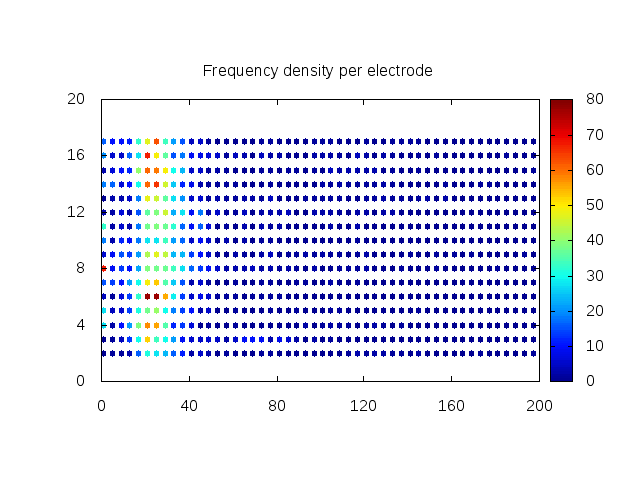
\includegraphics[width=0.4\linewidth]
{d1i.png} }}
	\qquad
	\subfloat[Preictal]
{{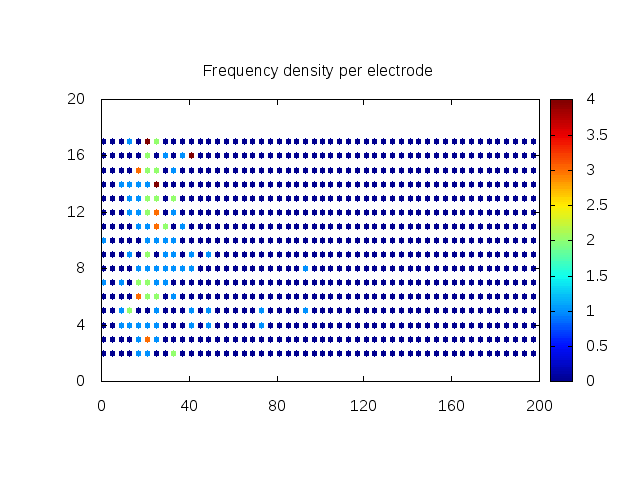
\includegraphics[width=0.4\linewidth]
{d1p.png} }}
	\caption{Heatmaps showing distribution of electrode-wise principal frequency for Dog1 data. x-axis represents frequency in Hertz.}
	\label{d1freq}
\end{figure}

\subsubsection{Fourier Spectra}
\label{spec}
Next we looked at the spectrum of amplitudes obtained from a Fourier decomposition on each electrode's signals. Here, we observe marked differences among preictal and interictal spectra for some particular electrodes. A few representative examples can be seen in figures \ref{d1e5spec} and \ref{d2e10spec}. For both cases shown here, the interictal plots are more peaked towards frequencies close to 0. Thus, we can use the vector of amplitudes across a range of frequencies, say 0-200 Hz as a feature for distinguishing between pre- and inter-ictal segments. 

As also mentioned in \ref{spec}, we take the vector of amplitudes obtained on Fourier decomposition of each electrode's signal and use it as a feature vector to train models. In \cite{lecun}, the use of patient-specific machine learning-based classifiers (support vector machines, logistic regression or convolutional neural networks) has been mentioned. 

As the size of such a feature vector can become very large (number of electrodes * number of frequencies), we use a low band pass filter. This is meaningful because we can observe from the fourier spectra shown in \ref{spec} that the amplitudes past a certain frequency (around 100 Hz) are almost 0. We do not expect sinusoidal waves of high frequency to show up in neural activity anyway.

\begin{figure}[H]
	\centering
	\subfloat[Interictal]
{{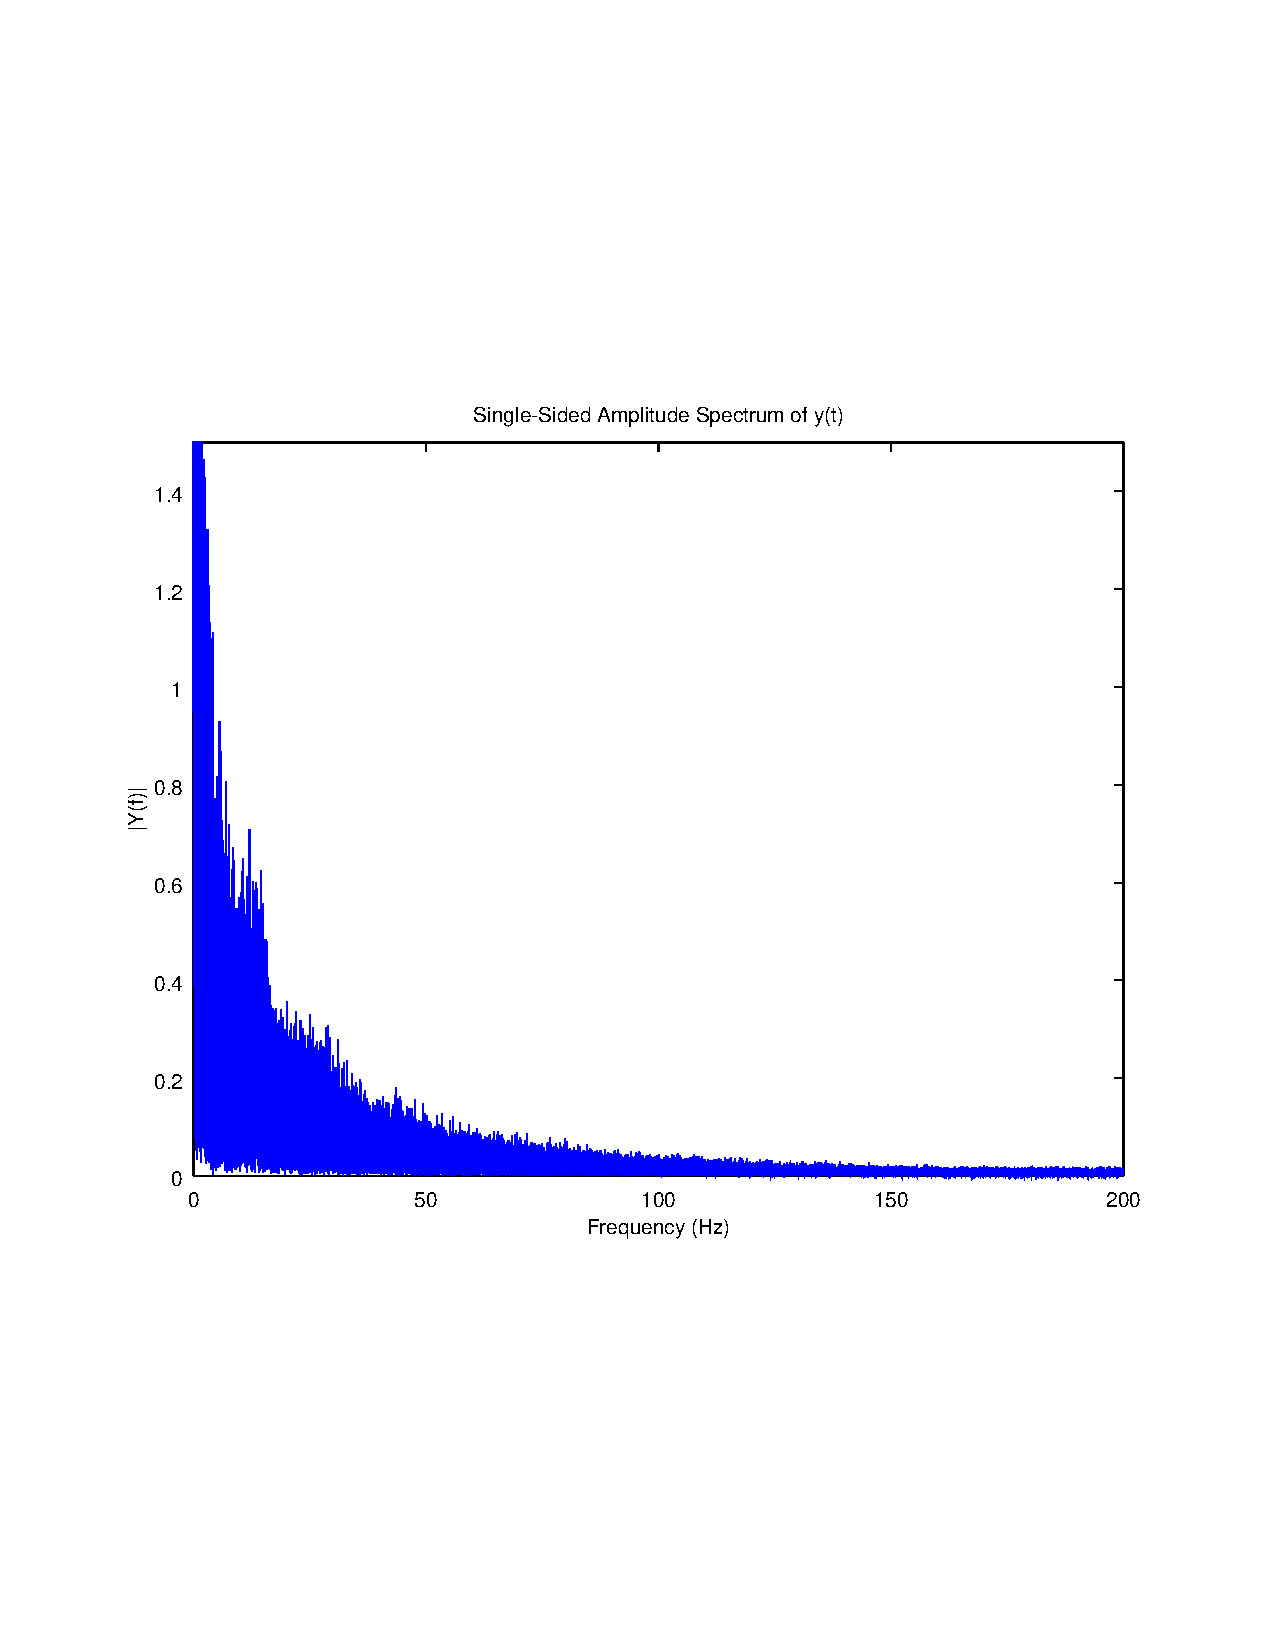
\includegraphics[width=0.4\linewidth]
{d1e5i11.pdf} }}
	\qquad
	\subfloat[Preictal]
{{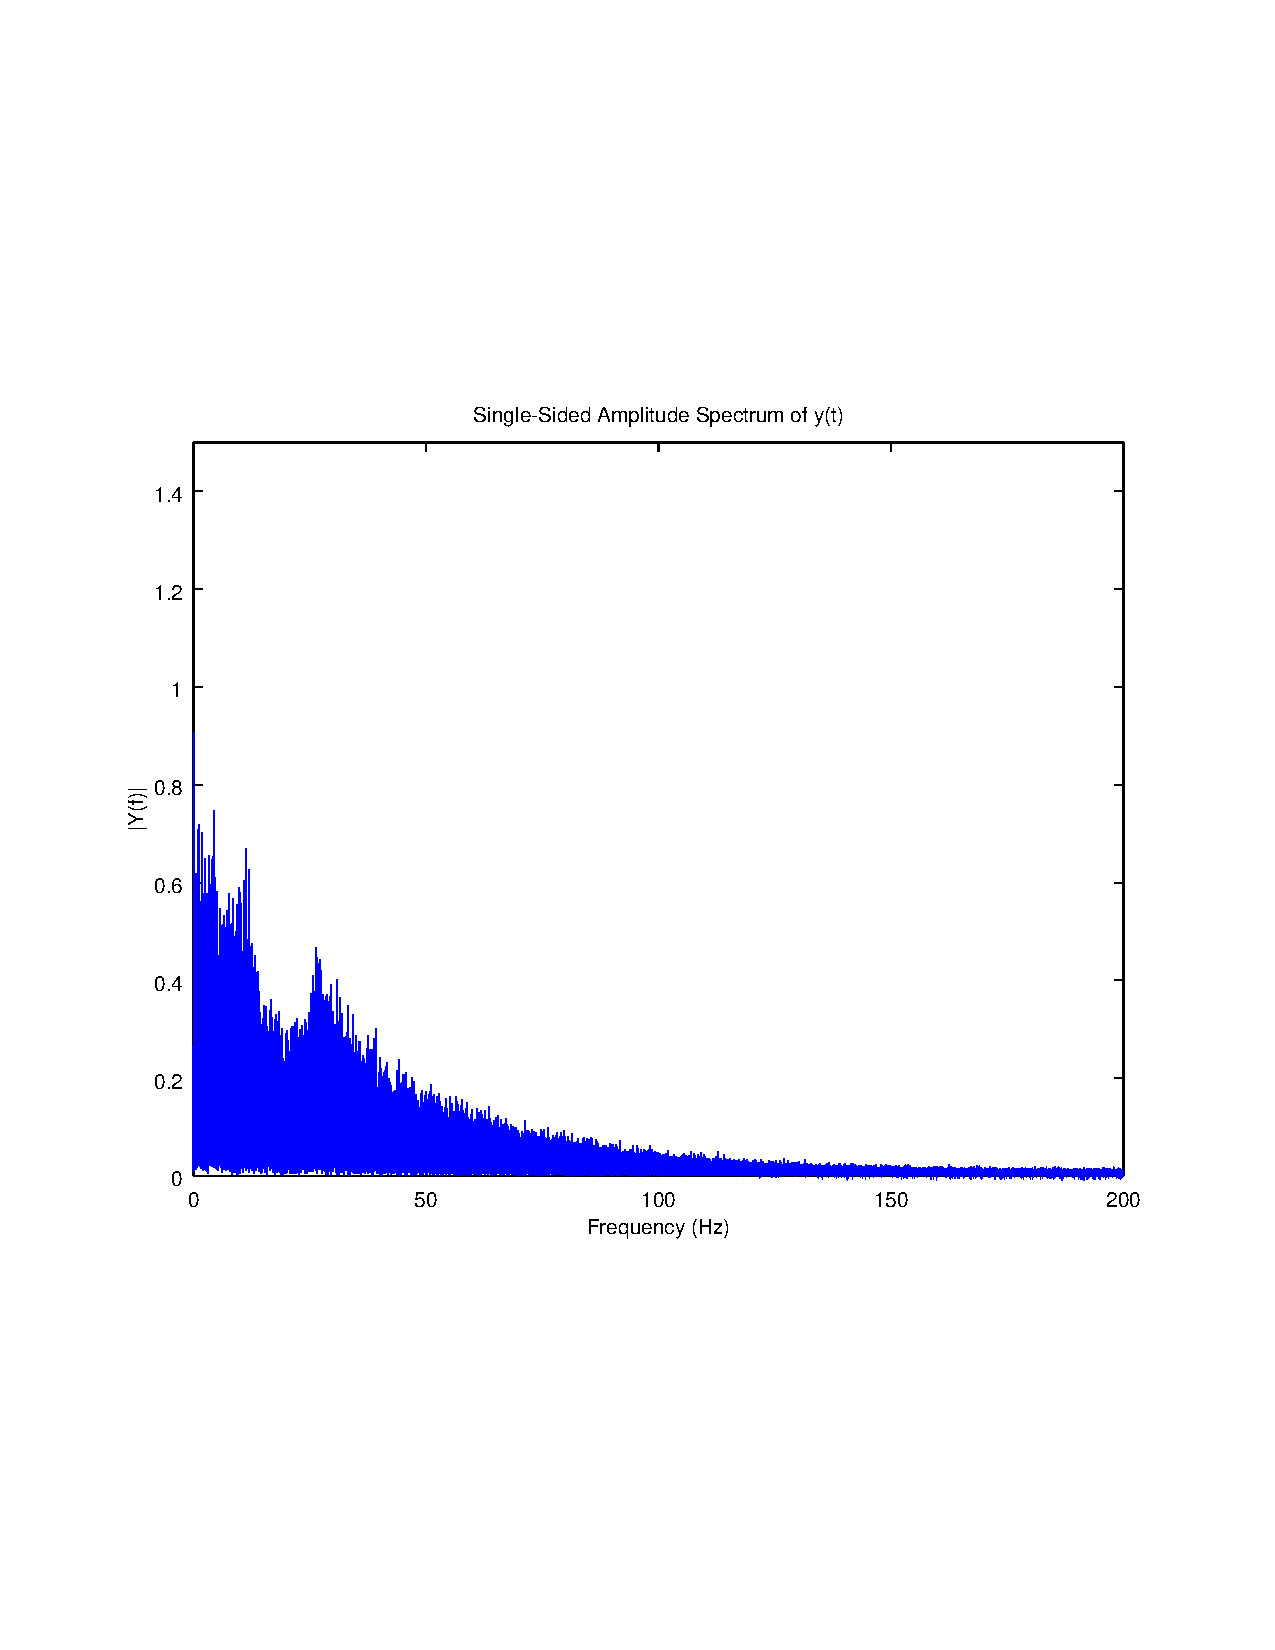
\includegraphics[width=0.4\linewidth]
{d1e5p23.pdf} }}
	\caption{Fourier spectra for the $5^{th}$ electrode in Dog1 data.}
	\label{d1e5spec}
\end{figure}

\begin{figure}[H]
	\centering
	\subfloat[Interictal]
{{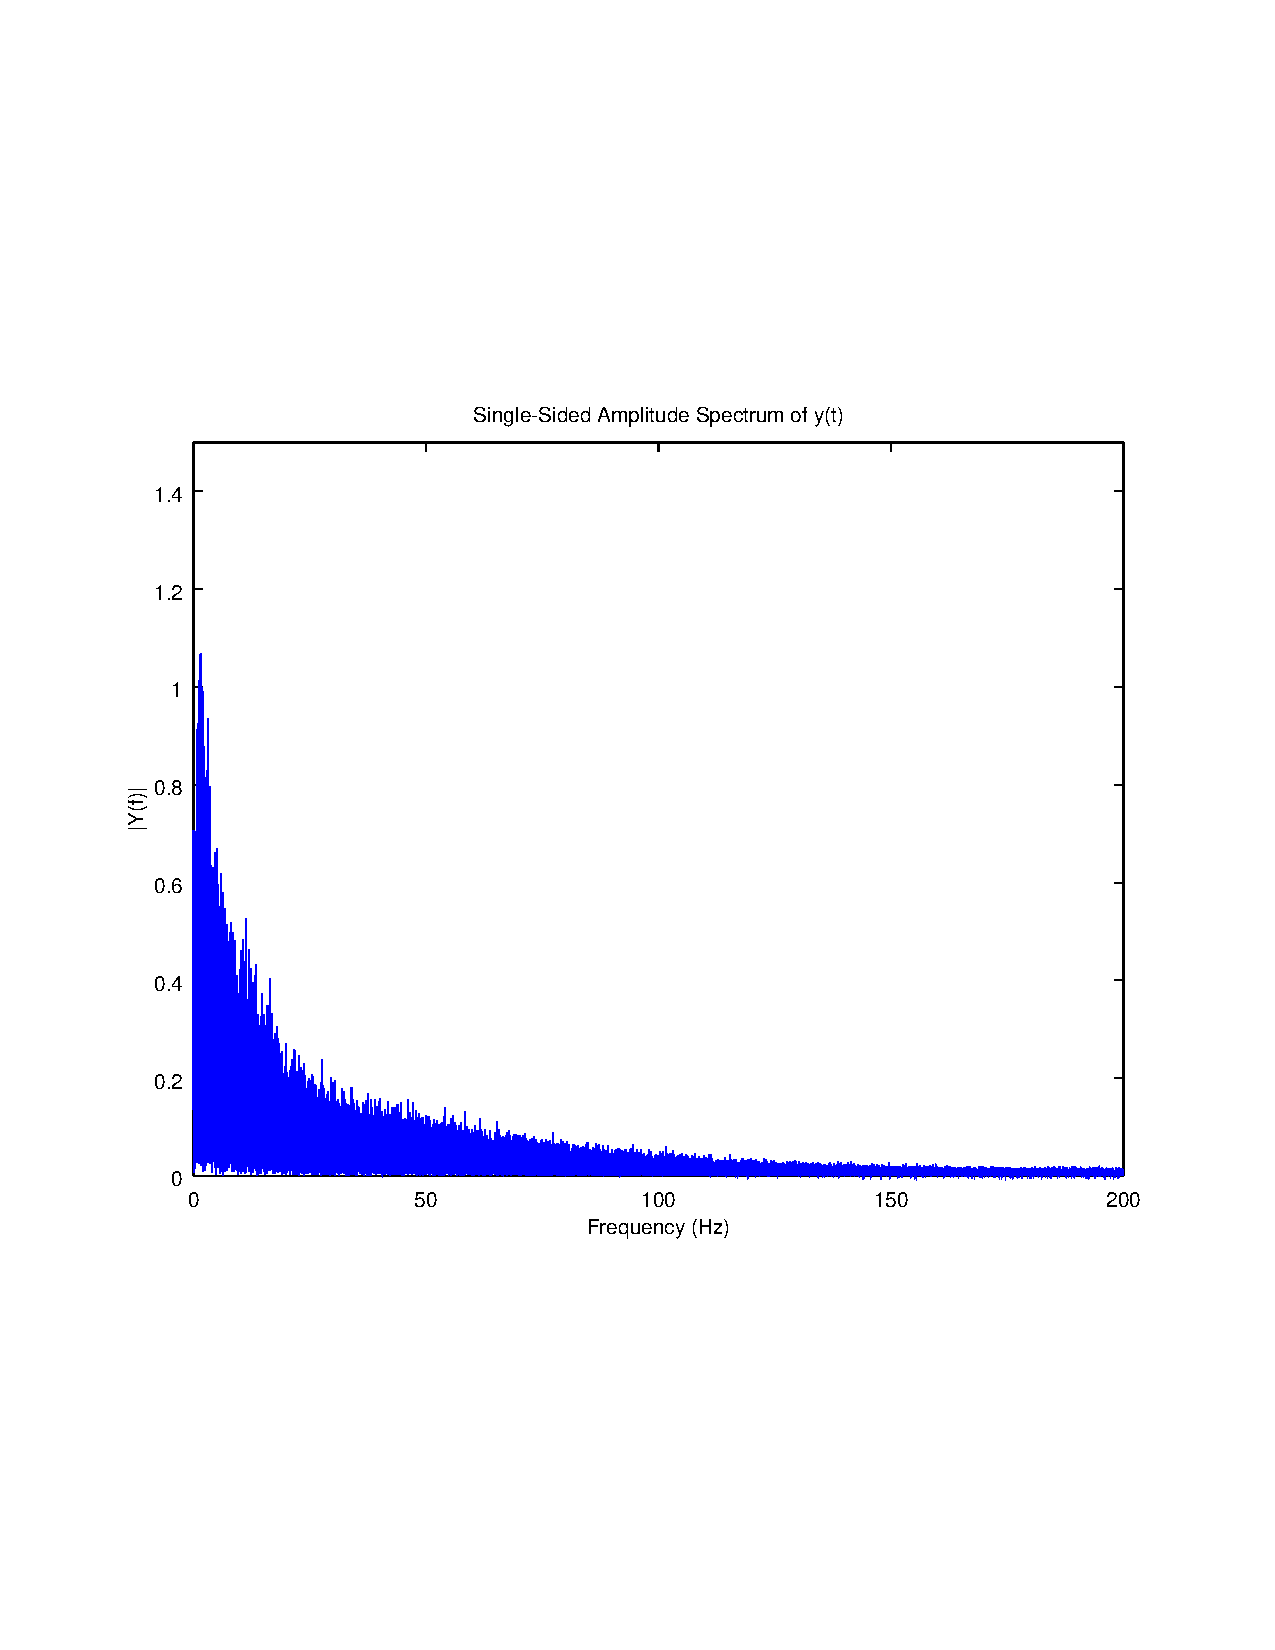
\includegraphics[width=0.4\linewidth]
{d2e10i1.pdf} }}
	\qquad
	\subfloat[Preictal]
{{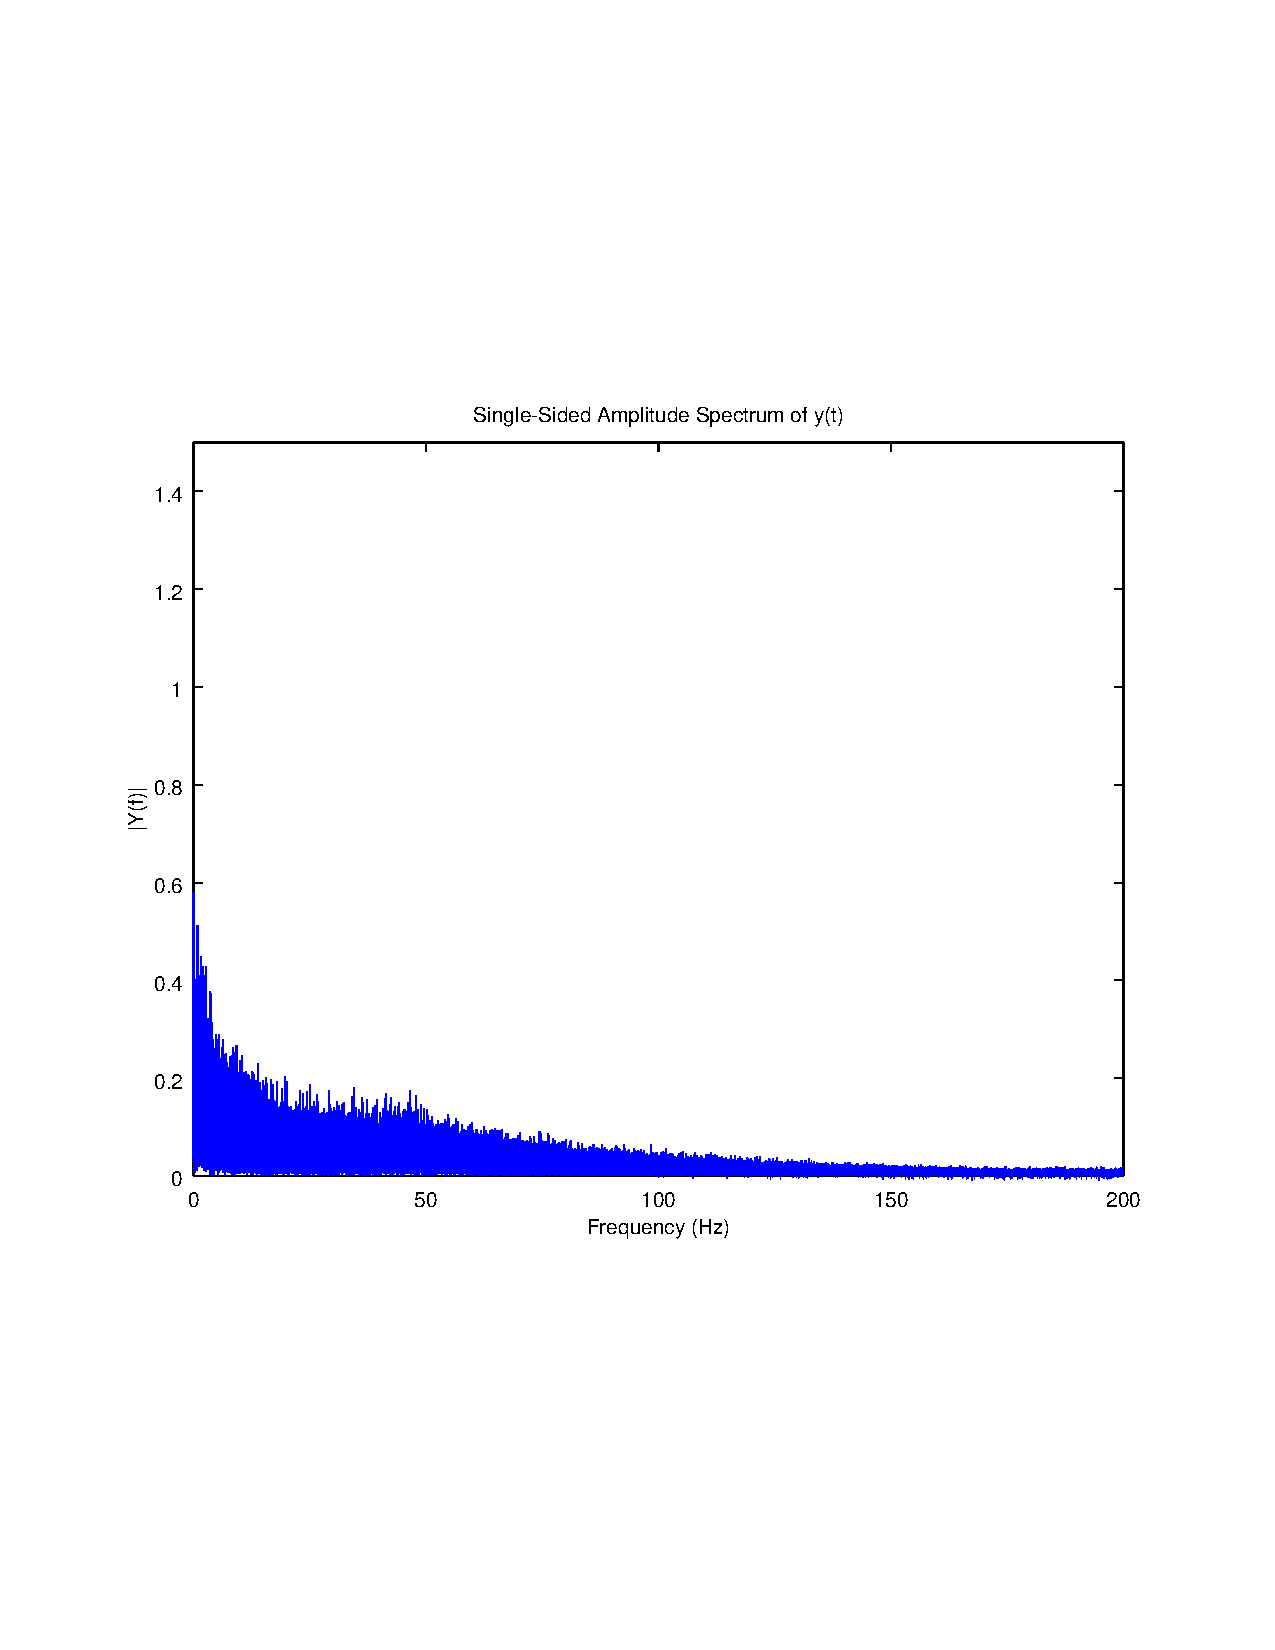
\includegraphics[width=0.4\linewidth]
{d2e10p1.pdf} }}
	\caption{Fourier spectra for the $10^{th}$ electrode in Dog2 data.}
	\label{d2e10spec}
\end{figure}

\subsubsection{Using bivariate features}
After filtering outliers, we plotted correlation heatmaps among electrode-pairs, looking at their principal frequencies, and obtained good distinction between the two classes of data. We therefore, plan to use such correlation matrices as bivariate features for our models, which is also supported in \cite{lecun}. In figure \ref{d1freqcorr}, we can see that there is more correlation among the electrodes in preictal segments, which is to be expected during a seizure.

\begin{figure}[H]
	\centering
	\subfloat[Interictal]
{{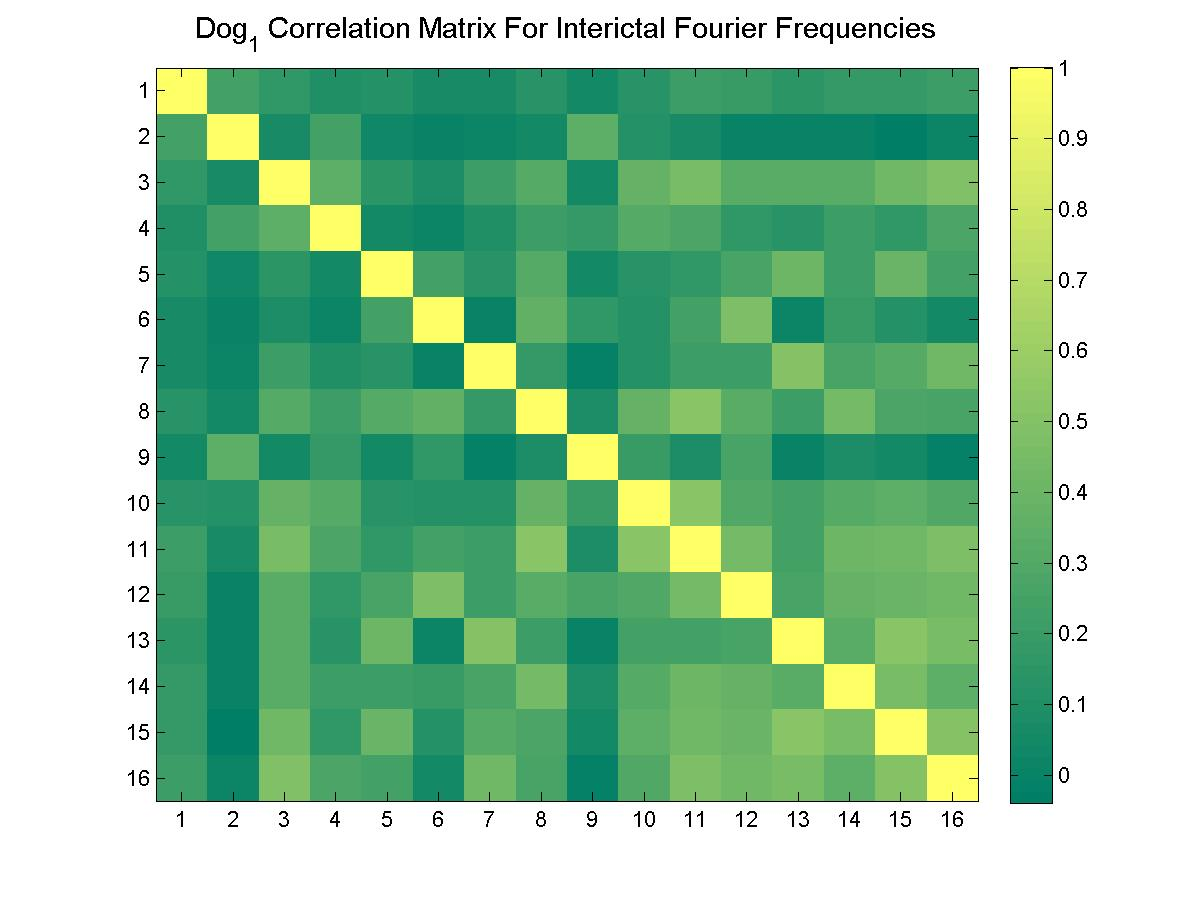
\includegraphics[width=0.4\linewidth]
{Dog1_InterictalFourierCorrelationPlot.jpg} }}
	\qquad
	\subfloat[Preictal]
{{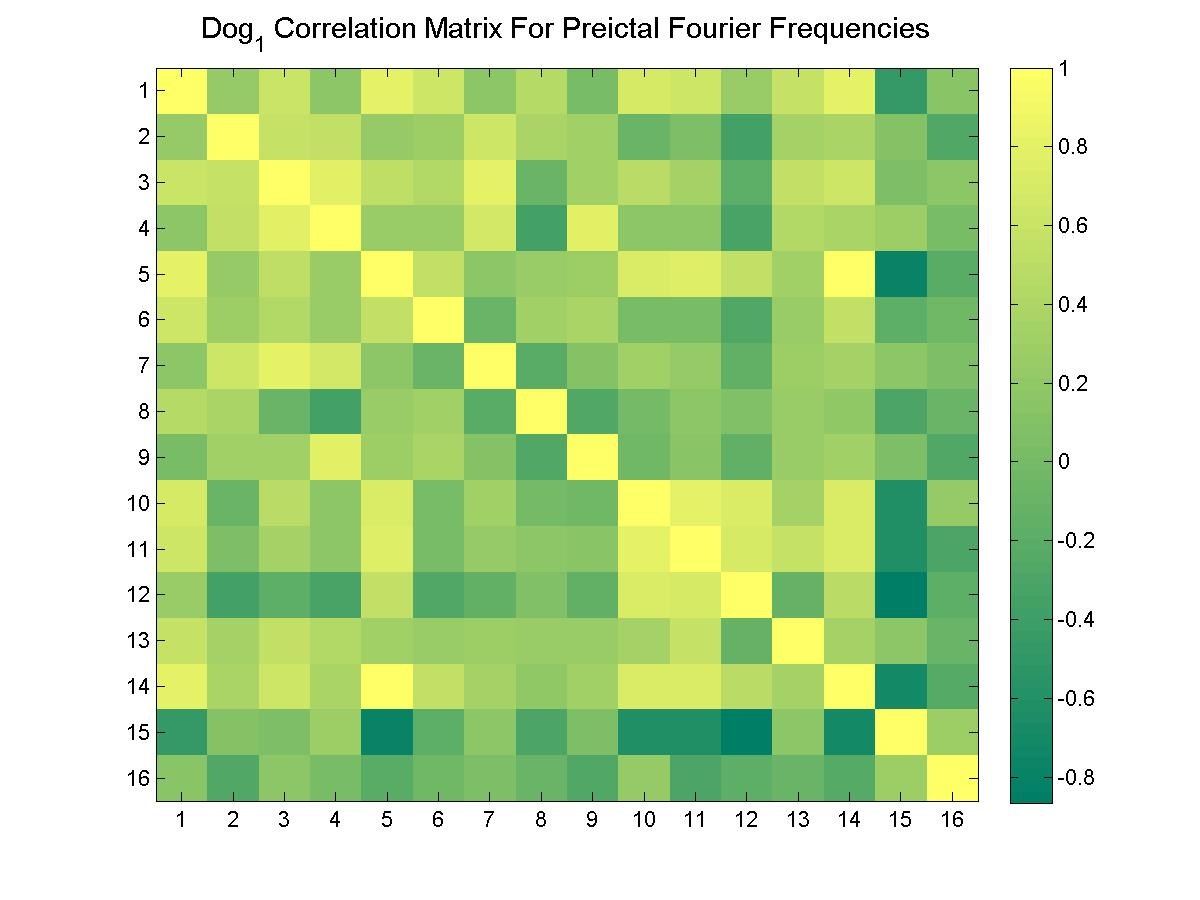
\includegraphics[width=0.4\linewidth]
{Dog1_PreictalFourierCorrelationPlot.jpg} }}
	\caption{Correlation heatmap among principal frequencies for different electrodes in Dog1 data}
	\label{d1freqcorr}
\end{figure}

\section{Experiments}

\subsection{Types Of Features Used}

The classifiers that we tried out used combinations of the following features for a subject with $E$ electrodes:

\begin{enumerate}
\item \textbf{Means} of the data readings of each electrode.
\item \textbf{Variances} of the data readings of each electrode.
\item \textbf{Correlation Coefficients} for each pair of electrodes. This is essentially the lower (or upper) triangle portion of the correlation coefficient matrix of a data clip.
\item \textbf{Fourier Frequencies: } The top few principal frequencies of the Fourier amplitude spectrum for an electrode's readings.
\item \textbf{Fourier Frequency Similarities: } For each pair of electrodes, the similarity between their 'top frequencies' vectors is calculated. This is done by observing the number of common frequencies (with a tolerance) in the two vectors.
\item \textbf{Fourier Amplitudes: } We apply a low band pass filter and restrict ourselves to the amplitudes of the first few frequencies. We get a vector of amplitudes for each electrode.
\item \textbf{Fourier Amplitude Vector Similarity: } To compare how similar two electrodes are based on their amplitude vectors, we have two approaches:
\begin{itemize}
\item \textbf{Cosine Similarity: } For each pair of electrodes, the similarity between the two amplitude vectors is calculated using the cosine similarity measure.
\item \textbf{Euclidean Distance: } For each pair of electrodes, the distance(and in a way, similarity) between the two amplitude vectors is calculated using the euclidean distance measure.
\end{itemize}
\end{enumerate}

\subsection{Testing Framework}
For testing purposes, we're using a K-Fold cross-validation approach. For each subject, the M training segments of interictal data and N segments of preictal data are divided into partitions of size $\frac{M}{K}, \frac{N}{K}$ respectively. Thus, we will have K subsamples that contain equal number of interictal and preictal training segments. \\
One of the subsamples is chosen for validation purposes while the rest are used to train the classifier. This is repeated for all K subsamples and we note down the average metric score. For this project, we're setting K=3 so that we have a decent number of preictal data segments for testing. 

The basic metric that could be used for evaluation is the average number of classification errors (or error percentage) of the classifier.

For our project, an important point to consider is that it is crucial for us to be able to predict the occurrence of a seizure given a preictal data segment (so that the patient may make preparations). False negatives (classifying a preictal segment as interictal) should be penalized more when compared to false positives(classifying an interictal segment as preictal). Thus, it is important for us to have a higher recall than precision. For that purpose we will be using the f-Measure metric (with higher weight on recall) $ = \frac{3PR}{2P + R} $ as a part of our evaluation.

For our evaluation, we define,

$$\text{Precision} = \frac{\text{Number of Accurate Preictal Predictions}}{\text{Number of Preictal Predictions}}$$

$$\text{Recall} = \frac{\text{Number of Accurate Preictal Predictions}}{\text{Number of Preictal Segments in the Test Set}}$$

$$\text{Error Percentage} = \frac{\text{Number of Misclassifications made} * 100}{\text{Number of Testing Data Segments}}$$

We've tried a couple of models for classification using basic features. For these models, our experimental set up is as shown in Table \ref{tab:data}.

\begin{table}[!htbp]
\centering
\begin{tabular}{*4c}
\toprule
Subject & Interictal data : Preictal data & $\#$ Training data & $\#$ Testing data\\
\midrule
Dog 1 & 480 : 24 & 336 & 168\\
Dog 2 & 500 : 42 & 361 & 181\\
Dog 3 & 1440 : 72 & 1008 & 504\\
Dog 4 & 804 : 97 & 601 & 300\\
Dog 5 & 450 : 30 & 320 & 160\\
Patient 1 & 50 : 18 & 45 & 23\\
Patient 2 & 42 : 18 & 40 & 20\\
\bottomrule
\end{tabular}
\caption{Data Used By The Models, during cross-validation}
\label{tab:data}
\end{table}

In Table \ref{tab:data}, the second column refers to the number of Interictal data segments we have vs the number of preictal data segments. Columns 3 \& 4 refer to the number of training and testing segments we will be using for our 3 fold cross validation framework.

It has to be noted that we will be building subject specific models (in terms of parameters). The underlying algorithm and feature extraction would remain same but while predicting for a given subject, we will only consider the relevant training data. We do not intend on building a `one size fits all' classifier. The merits of using patient specific classifiers have been studied in \cite{yunpark}.

\subsection{Bonehead Model}
For this model, we are considering the mean sample values for each electrode as the set of features for a data segment. For example, given a data segment of a subject with M electrodes, we would represent it with a 1 x M vector with each value representing the average data value for each electrode. \\
These data points are then fed to a Naive Bayes learner which generates a Gaussian Naive Bayes classifier.

The results of this classifier can be seen in Table \ref{tab:bonehead}.

\begin{table}[!htbp]
\centering
\resizebox{\linewidth}{!}{%
\begin{tabular}{c c c c c c c c c c c c c c}
\toprule
Subject & \multicolumn{4}{c}{Test on Fold 1} & \multicolumn{4}{c}{Test on Fold 2} & \multicolumn{4}{c}{Test on Fold 3} & MeanError\\
\midrule
 & Errors  & Precision & Recall  & f-Measure  &  Errors  & Precision & Recall & f-Measure	& Errors  & Precision & Recall & f-Measure\\
Dog 1 &  7.74\% & 0.27 & 0.38 & 0.33 &  12.5\% & 0.16 & 0.38 & 0.26 &  10.12\% & 0.15 & 0.25 & 0.21 & 10.12\%\\
Dog 2 &  10.5\% & 0.42 & 1.0 & 0.69 &  15.47\% & 0.28 & 0.64 & 0.45 &  9.39\% & 0.45 & 1.0 & 0.71 & 11.78\%\\
Dog 3 &  5.75\% & 0.0 & 0.0 & 0 &  4.56\% & 1.0 & 0.04 & 0.06 &  5.95\% & 0.0 & 0.0 & 0 & 5.42\%\\
Dog 4 &  10.33\% & 1.0 & 0.03 & 0.05 &  11.0\% & 0.0 & 0.0 & 0 &  11.33\% & 0.0 & 0.0 & 0 & 10.89\%\\
Dog 5 &  8.75\% & 0.36 & 0.5 & 0.44 &  8.13\% & 0.33 & 0.3 & 0.31 &  16.88\% & 0.16 & 0.4 & 0.27 & 11.25\%\\
Patient 1 &  34.78\% & 0.25 & 0.17 & 0.19 &  26.09\% & 0.0 & 0.0 & 0 &  21.74\% & 0.67 & 0.33 & 0.4 & 27.52\%\\
Patient 2 &  30.0\% & 0.5 & 0.17 & 0.21 &  50.0\% & 0.17 & 0.17 & 0.17 &  35.0\% & 0.0 & 0.0 & 0 & 38.35\%\\
\bottomrule
\end{tabular}
}
\caption{Performance of the bonehead model.}
\label{tab:bonehead}
\end{table}

\subsection{Regression Trees}
The bonehead model tries fitting all segments of a type using the same global parameters, which might not be a good idea if there actually are variations within a class. So, we tried the regression tree model which allows us to fit simple models to small partitions of the training data and hence, take into account local variations. 

We used the following combinations of features: 
\begin{enumerate}
\item \textbf{Variances and Correlation Coefficients :} This is our base set of features which we use for all the models that follow. We observe that this model beats the bonehead model with ease in terms of accuracy of prediction and recall. This is expected given that we're using more discriminating features.

\item \textbf{Variances, Correlation Coefficients, Top Fourier Frequencies :} We're including the top principal frequencies of each electrode's Fourier Spectrum. The performance of this model seems to be poor which can be attributed to the fact that the frequency values themselves aren't features that can differentiate between interictal and preictal samples.

\item \textbf{Variances, Correlation Coefficients, similarity between frequency vectors :} To solve the problems of the previous model, we try looking at how each pair of electrodes are correlated with each other with respect to their top principal frequencies. This is a bivariate feature and seems to be improving the accuracy of the classifier.

\item \textbf{Variances, Correlation Coefficients, Amplitude Vectors: } Adding the amplitude vectors to the base set of features improves the performance which suggests that the amplitude vectors are good features.

\item \textbf{Variances, Correlation Coefficients, Cosine Similarity between Amplitude Vectors: } Here we try introducing more bivariate features by including the cosine similarities between all pairs of amplitude vectors. This model outperforms the previous term which lends support to the claim that bivariate features are better features.

\item \textbf{Variances, Correlation Coefficients, Euclidean Distance between Amplitude Vectors :} This is similar to the previous model. Here, we're using the Euclidean distance between two amplitude vectors as a measure of similarity/dissimilarity between two electrodes.
\end{enumerate}

\subsection{SVM}
Next, we tried using the SVM classifier primarily because of the power of the classifier and the ability to use the Kernel trick which allows us to map our features to a high dimensional space. For our experiments, we used the linear kernel function and the RBF kernel function.

\subsubsection{Linear SVM}

We used the following combinations of features: 
\begin{enumerate}
\item \textbf{Variances, Correlation Coefficients, Top Fourier Frequencies :} Here, we use the top principal frequencies of each electrode's Fourier spectrum as features. This model performs better than the bonehead model.
\item \textbf{Variances, Correlation Coefficients, similarities between top frequency vectors :} In this model, we add bivariate features that measure the correlation between two electrodes on the basis of their frequency vectors. This results in a slightly better model when compared to the previous one.
\item \textbf{Variances, Correlation Coefficients, Amplitude Vectors:} Using the amplitude vectors of each electrode as features results in a model that outperforms the previous two models. This is further indication that the amplitude vectors tell us more about the data than the frequency vectors.
\item \textbf{Variances, Correlation Coefficients, Cosine Similarity between Amplitude Vectors:} 
\item \textbf{Variances, Correlation Coefficients, Euclidean Distance between Amplitude Vectors}
\end{enumerate}

In general, we observe that a linear SVM outperforms the regression tree classifier used before.


\subsubsection{RBF Kernel SVM}





\subsection{Ensemble Methods(Adaboost)}
Lastly, we tried using Ensemble methods (Adaboost) with decision stumps as the weak learner. The motivation for this is that boosting lets us learn complex decision boundaries by training a series of weak learners. 

Again, we used multiple combinations here too:

\begin{itemize}
\item \textbf{Variances, Correlation Coefficients and Fourier Frequencies Similarity:} 
\item \textbf{Variances, Correlation Coefficients and Amplitude Vectors}
\item \textbf{Variances, Correlation Coefficients and Cosine Similarity between Amplitude Vectors}
\item \textbf{Variances, Correlation Coefficients and Euclidean Distance between Amplitude Vectors}
\end{itemize}

\section{Conclusions}
What observations here ?

\section{Future Work}
Future Work (ICA D:)

\begin{thebibliography}{99}
\bibitem{lecun} Piotr Mirowski, Deepak Madhavan, Yann LeCun, Ruben Kuzniecky (2008) \textit{Classification of Patterns of EEG Synchronization for Seizure Prediction} IEEE Workshop on Machine Learning for Signal Processing.
\bibitem{arnhold} Klaus Lehnertz, Ralph G. Andrzejak, Jochen Arnhold, Thomas Kreuz (2001) \textit{Nonlinear EEG Analysis in Epilepsy: Its Possible Use for Interictal Focus Localization, Seizure Anticipation, and Prevention} Journal of Clinical Neurophysiology.
\bibitem{yunpark} Yun Park, Lan Luo, Keshab K. Parhi, and Theoden Netoff(2011) \textit{Seizure prediction with spectral power of EEG using cost-sensitive support vector machines}

\end{thebibliography}

\clearpage

\appendix
\section{Classifier Results}
The following tables are the results obtained upon each classifier and a combination of features on the dataset:

\begin{table}[!htbp]
\centering
\resizebox{\linewidth}{!}{%
\begin{tabular}{c c c c c c c c c c c c c c}
\toprule
Subject & \multicolumn{4}{c}{Test on Fold 1} & \multicolumn{4}{c}{Test on Fold 2} & \multicolumn{4}{c}{Test on Fold 3} & MeanError\\
\midrule
 & Errors  & Precision & Recall  & f-Measure  &  Errors  & Precision & Recall & f-Measure	& Errors  & Precision & Recall & f-Measure\\
Dog 1 &  11.90\% & 0.12 & 0.25 & 0.19 &  6.55\% & 0.20 & 0.12 & 0.14 &  5.95\% & 0.25 & 0.12 & 0.15 & 8.13\%\\
Dog 2 &  6.08\% & 0.59 & 0.71 & 0.67 &  9.94\% & 0.33 & 0.29 & 0.30 &  4.97\% & 0.69 & 0.64 & 0.66 & 7.00\%\\
Dog 3 &  6.75\% & 0.31 & 0.33 & 0.32 &  6.35\% & 0.33 & 0.33 & 0.33 &  6.55\% & 0.32 & 0.33 & 0.33 & 6.55\%\\
Dog 4 &  14.33\% & 0.32 & 0.28 & 0.29 &  15.00\% & 0.32 & 0.37 & 0.35 &  12.33\% & 0.42 & 0.40 & 0.41 & 13.89\%\\
Dog 5 &  7.50\% & 0.43 & 0.60 & 0.53 &  4.38\% & 0.64 & 0.70 & 0.68 &  6.25\% & 0.50 & 0.60 & 0.56 & 6.04\%\\
Patient 1 &  22.73\% & 0.56 & 0.83 & 0.71 &  27.27\% & 0.50 & 0.33 & 0.38 &  22.73\% & 0.55 & 1.00 & 0.78 & 24.24\%\\
Patient 2 &  25.00\% & 0.60 & 0.50 & 0.53 &  45.00\% & 0.00 & 0.00 & nan &  45.00\% & 0.29 & 0.33 & 0.32 & 38.33\%\\
\bottomrule
\end{tabular}
}
\caption{\textbf{Regression Tree} using Variances and Correlation Coefficients as Features}
\label{tab:regTreeVarCorr}
\end{table}


\begin{table}[!htbp]
\centering
\resizebox{\linewidth}{!}{%
\begin{tabular}{c c c c c c c c c c c c c c}
\toprule
Subject & \multicolumn{4}{c}{Test on Fold 1} & \multicolumn{4}{c}{Test on Fold 2} & \multicolumn{4}{c}{Test on Fold 3} & MeanError\\
\midrule
 & Errors  & Precision & Recall  & f-Measure  &  Errors  & Precision & Recall & f-Measure	& Errors  & Precision & Recall & f-Measure\\
Dog 1 &  13.69\% & 0.06 & 0.12 & 0.09 &  13.69\% & 0.06 & 0.12 & 0.09 &  10.12\% & 0.09 & 0.12 & 0.11 & 12.50\%\\
Dog 2 &  7.73\% & 0.50 & 0.36 & 0.39 &  8.84\% & 0.45 & 0.71 & 0.60 &  8.29\% & 0.33 & 0.07 & 0.10 & 8.29\%\\
Dog 3 &  7.74\% & 0.26 & 0.33 & 0.30 &  5.36\% & 0.40 & 0.25 & 0.29 &  7.74\% & 0.27 & 0.38 & 0.33 & 6.94\%\\
Dog 4 &  16.67\% & 0.20 & 0.19 & 0.19 &  17.00\% & 0.25 & 0.28 & 0.27 &  20.33\% & 0.18 & 0.25 & 0.22 & 18.00\%\\
Dog 5 &  11.25\% & 0.10 & 0.10 & 0.10 &  10.00\% & 0.29 & 0.40 & 0.35 &  11.25\% & 0.21 & 0.30 & 0.26 & 10.83\%\\
Patient 1 &  17.39\% & 0.67 & 0.67 & 0.67 &  34.78\% & 0.25 & 0.17 & 0.19 &  43.48\% & 0.00 & 0.00 & nan & 31.88\%\\
Patient 2 &  30.00\% & 0.50 & 0.17 & 0.21 &  45.00\% & 0.40 & 1.00 & 0.67 &  45.00\% & 0.29 & 0.33 & 0.32 & 40.00\%\\
\bottomrule
\end{tabular}
}
\caption{\textbf{Regression Tree} using Variances, Correlation Coefficients and Top Fourier Frequencies}
\label{tab:regTreeVarCorrFreq}
\end{table}


\begin{table}[!htbp]
\centering
\resizebox{\linewidth}{!}{%
\begin{tabular}{c c c c c c c c c c c c c c}
\toprule
Subject & \multicolumn{4}{c}{Test on Fold 1} & \multicolumn{4}{c}{Test on Fold 2} & \multicolumn{4}{c}{Test on Fold 3} & MeanError\\
\midrule
 & Errors  & Precision & Recall  & f-Measure  &  Errors  & Precision & Recall & f-Measure	& Errors  & Precision & Recall & f-Measure\\
Dog 1 &  8.33\% & 0.25 & 0.38 & 0.32 &  4.76\% & 0.50 & 0.25 & 0.30 &  10.71\% & 0.08 & 0.12 & 0.11 & 7.94\%\\
Dog 2 &  10.56\% & 0.35 & 0.43 & 0.40 &  7.22\% & 0.55 & 0.43 & 0.46 &  7.78\% & 0.50 & 0.50 & 0.50 & 8.52\%\\
Dog 3 &  4.76\% & 0.50 & 0.38 & 0.41 &  5.36\% & 0.43 & 0.42 & 0.42 &  4.96\% & 0.47 & 0.38 & 0.40 & 5.03\%\\
Dog 4 &  15.95\% & 0.21 & 0.19 & 0.19 &  11.96\% & 0.41 & 0.28 & 0.31 &  14.62\% & 0.34 & 0.37 & 0.36 & 14.17\%\\
Dog 5 &  8.75\% & 0.17 & 0.10 & 0.12 &  3.75\% & 0.75 & 0.60 & 0.64 &  6.88\% & 0.45 & 0.50 & 0.48 & 6.46\%\\
Patient 1 &  27.27\% & 0.50 & 0.50 & 0.50 &  13.64\% & 0.67 & 1.00 & 0.86 &  31.82\% & 0.43 & 0.50 & 0.47 & 24.24\%\\
Patient 2 &  30.00\% & 0.50 & 0.17 & 0.21 &  20.00\% & 0.62 & 0.83 & 0.75 &  15.00\% & 0.71 & 0.83 & 0.79 & 21.67\%\\
\bottomrule
\end{tabular}
}
\caption{\textbf{Regression Tree} using Variances, Correlation Coefficients and Frequency Similarity}
\label{tab:regTreeVarCorrFreqSim}
\end{table}


\begin{table}[!htbp]
\centering
\resizebox{\linewidth}{!}{%
\begin{tabular}{c c c c c c c c c c c c c c}
\toprule
Subject & \multicolumn{4}{c}{Test on Fold 1} & \multicolumn{4}{c}{Test on Fold 2} & \multicolumn{4}{c}{Test on Fold 3} & MeanError\\
\midrule
 & Errors  & Precision & Recall  & f-Measure  &  Errors  & Precision & Recall & f-Measure	& Errors  & Precision & Recall & f-Measure\\
Dog 1 &  11.31\% & 0.08 & 0.12 & 0.10 &  10.71\% & 0.08 & 0.12 & 0.11 &  7.14\% & 0.00 & 0.00 & nan & 9.72\%\\
Dog 2 &  2.76\% & 0.85 & 0.79 & 0.80 &  11.05\% & 0.38 & 0.64 & 0.52 &  7.73\% & 0.50 & 0.43 & 0.45 & 7.18\%\\
Dog 3 &  7.14\% & 0.20 & 0.17 & 0.18 &  7.14\% & 0.20 & 0.17 & 0.18 &  6.75\% & 0.27 & 0.25 & 0.26 & 7.01\%\\
Dog 4 &  14.95\% & 0.32 & 0.37 & 0.35 &  17.61\% & 0.23 & 0.28 & 0.26 &  18.60\% & 0.23 & 0.31 & 0.28 & 17.05\%\\
Dog 5 &  12.50\% & 0.08 & 0.10 & 0.09 &  9.38\% & 0.31 & 0.40 & 0.36 &  11.88\% & 0.20 & 0.30 & 0.26 & 11.25\%\\
Patient 1 &  56.52\% & 0.23 & 0.50 & 0.36 &  17.39\% & 0.67 & 0.67 & 0.67 &  17.39\% & 0.62 & 0.83 & 0.75 & 30.43\%\\
Patient 2 &  45.00\% & 0.33 & 0.50 & 0.43 &  35.00\% & 0.40 & 0.33 & 0.35 &  45.00\% & 0.29 & 0.33 & 0.32 & 41.67\%\\
\bottomrule
\end{tabular}
}
\caption{\textbf{Regression Tree} using Variances, Correlation Coefficients and Amplitude Vectors}
\label{tab:regTreeVarCorrAmps}
\end{table}


\begin{table}[!htbp]
\centering
\resizebox{\linewidth}{!}{%
\begin{tabular}{c c c c c c c c c c c c c c}
\toprule
Subject & \multicolumn{4}{c}{Test on Fold 1} & \multicolumn{4}{c}{Test on Fold 2} & \multicolumn{4}{c}{Test on Fold 3} & MeanError\\
\midrule
 & Errors  & Precision & Recall  & f-Measure  &  Errors  & Precision & Recall & f-Measure	& Errors  & Precision & Recall & f-Measure\\
Dog 1 &  10.71\% & 0.14 & 0.25 & 0.20 &  5.95\% & 0.00 & 0.00 & nan &  5.95\% & 0.25 & 0.12 & 0.15 & 7.54\%\\
Dog 2 &  6.63\% & 0.57 & 0.57 & 0.57 &  5.52\% & 0.62 & 0.71 & 0.68 &  6.08\% & 0.62 & 0.57 & 0.59 & 6.08\%\\
Dog 3 &  7.54\% & 0.28 & 0.38 & 0.34 &  6.75\% & 0.22 & 0.17 & 0.18 &  5.36\% & 0.44 & 0.46 & 0.45 & 6.55\%\\
Dog 4 &  13.29\% & 0.37 & 0.34 & 0.35 &  17.94\% & 0.21 & 0.25 & 0.23 &  13.62\% & 0.37 & 0.34 & 0.35 & 14.95\%\\
Dog 5 &  10.00\% & 0.31 & 0.50 & 0.42 &  6.88\% & 0.33 & 0.10 & 0.13 &  10.62\% & 0.27 & 0.40 & 0.34 & 9.17\%\\
Patient 1 &  26.09\% & 0.50 & 0.50 & 0.50 &  26.09\% & 0.50 & 0.17 & 0.21 &  13.04\% & 1.00 & 0.50 & 0.60 & 21.74\%\\
Patient 2 &  35.00\% & 0.40 & 0.33 & 0.35 &  30.00\% & 0.50 & 0.33 & 0.38 &  40.00\% & 0.33 & 0.33 & 0.33 & 35.00\%\\
\bottomrule
\end{tabular}
}
\caption{\textbf{Regression Tree} using variances, Correlation Coefficients and Cosine Similarity between Amplitude vectors}
\label{tab:regTreeVarCorrCosine}
\end{table}


\begin{table}[!htbp]
\centering
\resizebox{\linewidth}{!}{%
\begin{tabular}{c c c c c c c c c c c c c c}
\toprule
Subject & \multicolumn{4}{c}{Test on Fold 1} & \multicolumn{4}{c}{Test on Fold 2} & \multicolumn{4}{c}{Test on Fold 3} & MeanError\\
\midrule
 & Errors  & Precision & Recall  & f-Measure  &  Errors  & Precision & Recall & f-Measure	& Errors  & Precision & Recall & f-Measure\\
Dog 1 &  11.90\% & 0.00 & 0.00 & nan &  5.95\% & 0.38 & 0.38 & 0.38 &  7.14\% & 0.17 & 0.12 & 0.14 & 8.33\%\\
Dog 2 &  6.67\% & 0.60 & 0.43 & 0.47 &  3.89\% & 0.82 & 0.64 & 0.69 &  5.56\% & 0.67 & 0.57 & 0.60 & 5.37\%\\
Dog 3 &  4.56\% & 0.53 & 0.38 & 0.42 &  6.75\% & 0.32 & 0.38 & 0.36 &  6.55\% & 0.24 & 0.17 & 0.18 & 5.95\%\\
Dog 4 &  17.00\% & 0.23 & 0.25 & 0.24 &  17.33\% & 0.23 & 0.25 & 0.24 &  11.33\% & 0.47 & 0.59 & 0.54 & 15.22\%\\
Dog 5 &  6.25\% & 0.50 & 0.30 & 0.35 &  10.62\% & 0.18 & 0.20 & 0.19 &  5.62\% & 0.55 & 0.60 & 0.58 & 7.50\%\\
Patient 1 &  17.39\% & 0.62 & 0.83 & 0.75 &  8.70\% & 0.83 & 0.83 & 0.83 &  26.09\% & 0.50 & 0.50 & 0.50 & 17.39\%\\
Patient 2 &  25.00\% & 0.56 & 0.83 & 0.71 &  30.00\% & 0.50 & 0.67 & 0.60 &  40.00\% & 0.25 & 0.17 & 0.19 & 31.67\%\\
\bottomrule
\end{tabular}
}
\caption{\textbf{Regression Tree} using Variances, Correlation Coefficients and Euclidean Distance between Amplitude Vectors}
\label{tab:regTreeVarCorrEuclid}
\end{table}

\begin{table}[!htbp]
\centering
\resizebox{\linewidth}{!}{%
\begin{tabular}{c c c c c c c c c c c c c c}
\toprule
Subject & \multicolumn{4}{c}{Test on Fold 1} & \multicolumn{4}{c}{Test on Fold 2} & \multicolumn{4}{c}{Test on Fold 3} & MeanError\\
\midrule
 & Errors  & Precision & Recall  & f-Measure  &  Errors  & Precision & Recall & f-Measure	& Errors  & Precision & Recall & f-Measure\\
Dog 1 &  4.76\% & 0.50 & 0.12 & 0.17 &  5.36\% & 0.33 & 0.12 & 0.16 &  5.36\% & 0.00 & 0.00 & nan & 5.16\%\\
Dog 2 &  9.39\% & 0.29 & 0.14 & 0.17 &  9.39\% & 0.20 & 0.07 & 0.09 &  7.18\% & 0.56 & 0.36 & 0.41 & 8.66\%\\
Dog 3 &  6.94\% & 0.21 & 0.17 & 0.18 &  7.94\% & 0.25 & 0.33 & 0.30 &  6.94\% & 0.24 & 0.21 & 0.22 & 7.28\%\\
Dog 4 &  13.29\% & 0.38 & 0.37 & 0.37 &  14.95\% & 0.24 & 0.19 & 0.20 &  13.29\% & 0.35 & 0.25 & 0.27 & 13.84\%\\
Dog 5 &  4.38\% & 0.71 & 0.50 & 0.56 &  5.00\% & 1.00 & 0.20 & 0.27 &  6.25\% & 0.50 & 0.20 & 0.25 & 5.21\%\\
Patient 1 &  13.04\% & 1.00 & 0.50 & 0.60 &  8.70\% & 1.00 & 0.67 & 0.75 &  8.70\% & 1.00 & 0.67 & 0.75 & 10.14\%\\
Patient 2 &  25.00\% & 1.00 & 0.17 & 0.23 &  35.00\% & 0.44 & 0.67 & 0.57 &  30.00\% & 0.00 & 0.00 & nan & 30.00\%\\
\bottomrule
\end{tabular}
}
\caption{\textbf{Linear SVM} on Variances, Correlation Coefficients and Top Fourier Frequencies.}
\label{tab:svmVarCorrFreqs}
\end{table}


\begin{table}[!htbp]
\centering
\resizebox{\linewidth}{!}{%
\begin{tabular}{c c c c c c c c c c c c c c}
\toprule
Subject & \multicolumn{4}{c}{Test on Fold 1} & \multicolumn{4}{c}{Test on Fold 2} & \multicolumn{4}{c}{Test on Fold 3} & MeanError\\
\midrule
 & Errors  & Precision & Recall  & f-Measure  &  Errors  & Precision & Recall & f-Measure	& Errors  & Precision & Recall & f-Measure\\
Dog 1 &  5.95\% & 0.25 & 0.12 & 0.15 &  5.95\% & 0.33 & 0.25 & 0.27 &  5.95\% & 0.33 & 0.25 & 0.27 & 5.95\%\\
Dog 2 &  8.84\% & 0.44 & 0.50 & 0.48 &  7.73\% & 0.50 & 0.50 & 0.50 &  5.52\% & 0.67 & 0.57 & 0.60 & 7.37\%\\
Dog 3 &  6.35\% & 0.38 & 0.50 & 0.45 &  7.14\% & 0.30 & 0.38 & 0.35 &  6.94\% & 0.24 & 0.21 & 0.22 & 6.81\%\\
Dog 4 &  15.95\% & 0.28 & 0.31 & 0.30 &  18.27\% & 0.28 & 0.46 & 0.38 &  15.95\% & 0.29 & 0.31 & 0.30 & 16.72\%\\
Dog 5 &  1.88\% & 1.00 & 0.70 & 0.78 &  7.50\% & 0.33 & 0.20 & 0.23 &  5.62\% & 0.57 & 0.40 & 0.44 & 5.00\%\\
Patient 1 &  4.35\% & 1.00 & 0.83 & 0.88 &  8.70\% & 0.83 & 0.83 & 0.83 &  8.70\% & 1.00 & 0.67 & 0.75 & 7.25\%\\
Patient 2 &  35.00\% & 0.33 & 0.17 & 0.20 &  25.00\% & 0.67 & 0.33 & 0.40 &  20.00\% & 0.67 & 0.67 & 0.67 & 26.67\%\\
\bottomrule
\end{tabular}
}
\caption{\textbf{Linear SVM} on Variances, Correlation Coefficients and Similarities between the top frequency vectors.}
\label{tab:svmVarCorrFreqSim}
\end{table}


\begin{table}[!htbp]
\centering
\resizebox{\linewidth}{!}{%
\begin{tabular}{c c c c c c c c c c c c c c}
\toprule
Subject & \multicolumn{4}{c}{Test on Fold 1} & \multicolumn{4}{c}{Test on Fold 2} & \multicolumn{4}{c}{Test on Fold 3} & MeanError\\
\midrule
 & Errors  & Precision & Recall  & f-Measure  &  Errors  & Precision & Recall & f-Measure	& Errors  & Precision & Recall & f-Measure\\
Dog 1 &  4.76\% & 0.00 & 0.00 & nan &  4.76\% & 0.00 & 0.00 & nan &  5.95\% & 0.00 & 0.00 & nan & 5.16\%\\
Dog 2 &  6.63\% & 1.00 & 0.14 & 0.20 &  7.73\% & 0.00 & 0.00 & nan &  7.18\% & 1.00 & 0.07 & 0.10 & 7.18\%\\
Dog 3 &  4.37\% & 0.67 & 0.17 & 0.22 &  3.97\% & 0.70 & 0.29 & 0.36 &  4.17\% & 0.80 & 0.17 & 0.23 & 4.17\%\\
Dog 4 &  9.33\% & 0.62 & 0.31 & 0.37 &  10.00\% & 0.60 & 0.28 & 0.34 &  11.00\% & 0.47 & 0.22 & 0.26 & 10.11\%\\
Dog 5 &  5.62\% & 1.00 & 0.10 & 0.14 &  5.00\% & 1.00 & 0.20 & 0.27 &  4.38\% & 0.80 & 0.40 & 0.48 & 5.00\%\\
Patient 1 &  13.04\% & 1.00 & 0.50 & 0.60 &  4.35\% & 1.00 & 0.83 & 0.88 &  0.00\% & 1.00 & 1.00 & 1.00 & 5.80\%\\
Patient 2 &  30.00\% & 0.50 & 0.17 & 0.21 &  25.00\% & 0.67 & 0.33 & 0.40 &  20.00\% & 0.75 & 0.50 & 0.56 & 25.00\%\\
\bottomrule
\end{tabular}
}
\caption{\textbf{Linear SVM} on Variance, Correlation Coefficients and Amplitude Vectors}
\label{tab:svmVarCorrAmps}
\end{table}

\begin{table}[!htbp]
\centering
\resizebox{\linewidth}{!}{%
\begin{tabular}{c c c c c c c c c c c c c c}
\toprule
Subject & \multicolumn{4}{c}{Test on Fold 1} & \multicolumn{4}{c}{Test on Fold 2} & \multicolumn{4}{c}{Test on Fold 3} & MeanError\\
\midrule
 & Errors  & Precision & Recall  & f-Measure  &  Errors  & Precision & Recall & f-Measure	& Errors  & Precision & Recall & f-Measure\\
Dog 1 &  5.36\% & 0.44 & 0.50 & 0.48 &  6.55\% & 0.29 & 0.25 & 0.26 &  4.17\% & 0.60 & 0.38 & 0.43 & 5.36\%\\
Dog 2 &  4.44\% & 0.71 & 0.71 & 0.71 &  5.00\% & 0.69 & 0.64 & 0.66 &  4.44\% & 0.69 & 0.79 & 0.75 & 4.63\%\\
Dog 3 &  6.35\% & 0.32 & 0.29 & 0.30 &  5.95\% & 0.38 & 0.42 & 0.41 &  5.75\% & 0.42 & 0.54 & 0.49 & 6.02\%\\
Dog 4 &  15.95\% & 0.28 & 0.31 & 0.30 &  12.62\% & 0.41 & 0.40 & 0.40 &  14.62\% & 0.35 & 0.40 & 0.38 & 14.40\%\\
Dog 5 &  5.00\% & 0.60 & 0.60 & 0.60 &  1.88\% & 1.00 & 0.70 & 0.78 &  3.75\% & 0.83 & 0.50 & 0.58 & 3.54\%\\
Patient 1 &  4.55\% & 1.00 & 0.83 & 0.88 &  9.09\% & 1.00 & 0.67 & 0.75 &  0.00\% & 1.00 & 1.00 & 1.00 & 4.55\%\\
Patient 2 &  40.00\% & 0.38 & 0.50 & 0.45 &  20.00\% & 1.00 & 0.33 & 0.43 &  30.00\% & 0.50 & 0.33 & 0.38 & 30.00\%\\
\bottomrule
\end{tabular}
}
\caption{\textbf{Linear SVM} on Variances, Correlation Coefficients and Cosine Similarity between Amplitude Vectors.}
\label{tab:svmVarCorrCosine}
\end{table}

\begin{table}[!htbp]
\centering
\resizebox{\linewidth}{!}{%
\begin{tabular}{c c c c c c c c c c c c c c}
\toprule
Subject & \multicolumn{4}{c}{Test on Fold 1} & \multicolumn{4}{c}{Test on Fold 2} & \multicolumn{4}{c}{Test on Fold 3} & MeanError\\
\midrule
 & Errors  & Precision & Recall  & f-Measure  &  Errors  & Precision & Recall & f-Measure	& Errors  & Precision & Recall & f-Measure\\
Dog 1 &  7.74\% & 0.33 & 0.62 & 0.48 &  6.55\% & 0.33 & 0.38 & 0.36 &  4.17\% & 0.67 & 0.25 & 0.32 & 6.15\%\\
Dog 2 &  3.89\% & 0.77 & 0.71 & 0.73 &  3.33\% & 0.83 & 0.71 & 0.75 &  0.00\% & 1.00 & 1.00 & 1.00 & 2.41\%\\
Dog 3 &  3.77\% & 0.59 & 0.71 & 0.66 &  4.17\% & 0.56 & 0.58 & 0.58 &  4.37\% & 0.54 & 0.54 & 0.54 & 4.10\%\\
Dog 4 &  15.00\% & 0.33 & 0.40 & 0.38 &  13.33\% & 0.39 & 0.40 & 0.40 &  11.67\% & 0.47 & 0.62 & 0.56 & 13.33\%\\
Dog 5 &  3.12\% & 0.73 & 0.80 & 0.77 &  3.12\% & 0.86 & 0.60 & 0.67 &  2.50\% & 0.75 & 0.90 & 0.84 & 2.92\%\\
Patient 1 &  13.04\% & 1.00 & 0.50 & 0.60 &  8.70\% & 0.83 & 0.83 & 0.83 &  4.35\% & 0.86 & 1.00 & 0.95 & 8.70\%\\
Patient 2 &  40.00\% & 0.38 & 0.50 & 0.45 &  45.00\% & 0.29 & 0.33 & 0.32 &  35.00\% & 0.43 & 0.50 & 0.47 & 40.00\%\\
\bottomrule
\end{tabular}
}
\caption{\textbf{Linear SVM} on Variances, Correlation Coefficients and Euclidean Distance between Amplitude Vectors.}
\label{tab:svmVarCorrEuclid}
\end{table}

\begin{table}[!htbp]
\centering
\resizebox{\linewidth}{!}{%
\begin{tabular}{c c c c c c c c c c c c c c}
\toprule
Subject & \multicolumn{4}{c}{Test on Fold 1} & \multicolumn{4}{c}{Test on Fold 2} & \multicolumn{4}{c}{Test on Fold 3} & MeanError\\
\midrule
 & Errors  & Precision & Recall  & f-Measure  &  Errors  & Precision & Recall & f-Measure	& Errors  & Precision & Recall & f-Measure\\
Dog 1 &  4.76\% & 0.00 & 0.00 & nan &  4.17\% & 0.67 & 0.25 & 0.32 &  5.95\% & 0.25 & 0.12 & 0.15 & 4.96\%\\
Dog 2 &  0.55\% & 1.00 & 0.93 & 0.95 &  3.31\% & 0.90 & 0.64 & 0.71 &  3.31\% & 0.83 & 0.71 & 0.75 & 2.39\%\\
Dog 3 &  3.37\% & 0.89 & 0.33 & 0.42 &  2.78\% & 0.86 & 0.50 & 0.58 &  3.57\% & 0.80 & 0.33 & 0.41 & 3.24\%\\
Dog 4 &  10.30\% & 0.53 & 0.25 & 0.30 &  7.31\% & 0.81 & 0.40 & 0.48 &  9.63\% & 0.61 & 0.34 & 0.40 & 9.08\%\\
Dog 5 &  2.50\% & 1.00 & 0.60 & 0.69 &  5.00\% & 0.62 & 0.50 & 0.54 &  4.38\% & 0.71 & 0.50 & 0.56 & 3.96\%\\
Patient 1 &  4.35\% & 1.00 & 0.83 & 0.88 &  17.39\% & 1.00 & 0.33 & 0.43 &  13.04\% & 0.80 & 0.67 & 0.71 & 11.59\%\\
Patient 2 &  40.00\% & 0.33 & 0.33 & 0.33 &  40.00\% & 0.00 & 0.00 & nan &  15.00\% & 1.00 & 0.50 & 0.60 & 31.67\%\\
\bottomrule
\end{tabular}
}
\caption{\textbf{Adaboost} with Variance, Correlation Coefficients and Frequency Similarities.}
\label{tab:adaVarCorrFreqSim}
\end{table}

\begin{table}[!htbp]
\centering
\resizebox{\linewidth}{!}{%
\begin{tabular}{c c c c c c c c c c c c c c}
\toprule
Subject & \multicolumn{4}{c}{Test on Fold 1} & \multicolumn{4}{c}{Test on Fold 2} & \multicolumn{4}{c}{Test on Fold 3} & MeanError\\
\midrule
 & Errors  & Precision & Recall  & f-Measure  &  Errors  & Precision & Recall & f-Measure	& Errors  & Precision & Recall & f-Measure\\
Dog 1 &  4.76\% & 0.00 & 0.00 & nan &  4.76\% & 0.00 & 0.00 & nan &  4.76\% & 0.00 & 0.00 & nan & 4.76\%\\
Dog 2 &  5.52\% & 0.70 & 0.50 & 0.55 &  4.42\% & 1.00 & 0.43 & 0.53 &  4.97\% & 0.78 & 0.50 & 0.57 & 4.97\%\\
Dog 3 &  4.17\% & 0.80 & 0.17 & 0.23 &  4.56\% & 1.00 & 0.04 & 0.06 &  4.56\% & 0.67 & 0.08 & 0.12 & 4.43\%\\
Dog 4 &  9.97\% & 0.60 & 0.19 & 0.24 &  11.63\% & 0.33 & 0.09 & 0.12 &  13.29\% & 0.23 & 0.09 & 0.12 & 11.63\%\\
Dog 5 &  5.00\% & 1.00 & 0.20 & 0.27 &  4.38\% & 1.00 & 0.30 & 0.39 &  5.62\% & 1.00 & 0.10 & 0.14 & 5.00\%\\
Patient 1 &  30.43\% & 0.44 & 0.67 & 0.57 &  17.39\% & 0.75 & 0.50 & 0.56 &  34.78\% & 0.25 & 0.17 & 0.19 & 27.54\%\\
Patient 2 &  25.00\% & 0.67 & 0.33 & 0.40 &  15.00\% & 0.80 & 0.67 & 0.71 &  35.00\% & 0.00 & 0.00 & nan & 25.00\%\\
\bottomrule
\end{tabular}
}
\caption{\textbf{Adaboost} with Variance, Correlation Coefficients and Amplitudes.}
\label{tab:adaVarCorrAmps}
\end{table}

\begin{table}[!htbp]
\centering
\resizebox{\linewidth}{!}{%
\begin{tabular}{c c c c c c c c c c c c c c}
\toprule
Subject & \multicolumn{4}{c}{Test on Fold 1} & \multicolumn{4}{c}{Test on Fold 2} & \multicolumn{4}{c}{Test on Fold 3} & MeanError\\
\midrule
 & Errors  & Precision & Recall  & f-Measure  &  Errors  & Precision & Recall & f-Measure	& Errors  & Precision & Recall & f-Measure\\
Dog 1 &  5.36\% & 0.00 & 0.00 & nan &  4.76\% & 0.00 & 0.00 & nan &  4.17\% & 1.00 & 0.12 & 0.18 & 4.76\%\\
Dog 2 &  3.87\% & 0.82 & 0.64 & 0.69 &  3.31\% & 0.75 & 0.86 & 0.82 &  4.42\% & 0.88 & 0.50 & 0.58 & 3.87\%\\
Dog 3 &  4.17\% & 0.62 & 0.33 & 0.39 &  3.17\% & 0.90 & 0.38 & 0.47 &  3.57\% & 1.00 & 0.25 & 0.33 & 3.64\%\\
Dog 4 &  14.33\% & 0.18 & 0.09 & 0.11 &  11.33\% & 0.45 & 0.15 & 0.20 &  11.67\% & 0.40 & 0.19 & 0.23 & 12.44\%\\
Dog 5 &  3.12\% & 0.78 & 0.70 & 0.72 &  5.00\% & 0.67 & 0.40 & 0.46 &  3.75\% & 1.00 & 0.40 & 0.50 & 3.96\%\\
Patient 1 &  4.35\% & 1.00 & 0.83 & 0.88 &  17.39\% & 0.75 & 0.50 & 0.56 &  13.04\% & 0.80 & 0.67 & 0.71 & 11.59\%\\
Patient 2 &  25.00\% & 0.57 & 0.67 & 0.63 &  30.00\% & 0.50 & 0.33 & 0.38 &  25.00\% & 0.60 & 0.50 & 0.53 & 26.67\%\\
\bottomrule
\end{tabular}
}
\caption{\textbf{Adaboost} with Variance, Correlation Coefficients and Cosine Similarities between Amplitude Vectors}
\label{tab:adaVarCorrCosine}
\end{table}

\begin{table}[!htbp]
\centering
\resizebox{\linewidth}{!}{%
\begin{tabular}{c c c c c c c c c c c c c c}
\toprule
Subject & \multicolumn{4}{c}{Test on Fold 1} & \multicolumn{4}{c}{Test on Fold 2} & \multicolumn{4}{c}{Test on Fold 3} & MeanError\\
\midrule
 & Errors  & Precision & Recall  & f-Measure  &  Errors  & Precision & Recall & f-Measure	& Errors  & Precision & Recall & f-Measure\\
Dog 1 &  4.17\% & 0.67 & 0.25 & 0.32 &  4.76\% & 0.00 & 0.00 & nan &  4.76\% & 0.50 & 0.12 & 0.17 & 4.56\%\\
Dog 2 &  3.33\% & 0.75 & 0.86 & 0.82 &  3.33\% & 0.90 & 0.64 & 0.71 &  3.33\% & 0.83 & 0.71 & 0.75 & 3.33\%\\
Dog 3 &  2.78\% & 0.86 & 0.50 & 0.58 &  4.37\% & 0.62 & 0.21 & 0.27 &  3.57\% & 0.80 & 0.33 & 0.41 & 3.57\%\\
Dog 4 &  10.96\% & 0.46 & 0.19 & 0.23 &  9.30\% & 0.70 & 0.22 & 0.28 &  11.63\% & 0.44 & 0.22 & 0.26 & 10.63\%\\
Dog 5 &  3.75\% & 1.00 & 0.40 & 0.50 &  1.25\% & 0.90 & 0.90 & 0.90 &  3.12\% & 0.86 & 0.60 & 0.67 & 2.71\%\\
Patient 1 &  4.55\% & 1.00 & 0.83 & 0.88 &  18.18\% & 0.67 & 0.67 & 0.67 &  18.18\% & 1.00 & 0.33 & 0.43 & 13.64\%\\
Patient 2 &  25.00\% & 0.67 & 0.33 & 0.40 &  40.00\% & 0.38 & 0.50 & 0.45 &  35.00\% & 0.43 & 0.50 & 0.47 & 33.33\%\\
\bottomrule
\end{tabular}
}
\caption{\textbf{Adaboost} with Variance, Correlation Coefficients and Euclidean Distances between Amplitude Vectors}
\label{tab:adaVarCorrEuclid}
\end{table}

aaaaa

\end{document}